



\documentclass[letterpaper,12pt,oneside]{book}
\usepackage[utf8]{inputenc}
%\usepackage[a4paper,includeall,bindingoffset=0cm,margin=2cm,marginparsep=0cm,marginparwidth=0cm]{geometry}
\usepackage[top=1in, left=0.9in, right=1.25in, bottom=1in]{geometry}
\usepackage{bachelorstitlepageUNAM}
\usepackage{url}
\usepackage[T1]{fontenc}
\usepackage[spanish,es-nodecimaldot,es-tabla]{babel}
\usepackage{csquotes}
\usepackage{amsmath}
\usepackage{amsfonts}
\usepackage{amssymb} 
\usepackage{graphicx}
\usepackage[table]{xcolor}
\usepackage{tikz}
\usepackage{tocloft}
\graphicspath{{./figs/}}
\usepackage{setspace}
\usepackage{comment}
\usepackage{hyperref}
%\usepackage{showkeys}

\urlstyle{same}
\hypersetup{
   colorlinks=true,
   urlcolor=cyan,
   linkcolor=black,
   citecolor=black,
   filecolor=magenta,
   pdftitle={unidad teorica},
   pdfpagemode=FullScreen,
}
%\usepackage[natbibapa]{apacite}
\usepackage[font=scriptsize,labelfont=bf]{caption}
%\usepackage[round]{natbib}
\usepackage{linguex}

\usepackage[backend=biber, style=authoryear, sorting=ynt, sortcites]{biblatex}
\addbibresource{predoc.bib}
\usepackage{endnotes}
%\renewcommand\cftsecpresnum{\S}
%\renewcommand\cftsubsecpresnum{\S}

%%%%%%%%%%%%%%%%%%%%%%%%%%%%%

% Modificación de la plantilla original de esta url: 
% https://es.overleaf.com/latex/templates/tesis-unam-ingenieria-energia/kfffjrxcckdp

% Adaptada por Carlos Rodríguez Díaz para el CIC IPN.
% Cualquier sugerencia, corrección o comentario a: amnet04@gmail.com

% A continuación los comentarios de la plantilla original:

% Comparto una plantilla para la PORTADA que us\'e en mi t\'esis
% basada en el dise\~no gen\'erico que se usa en la Facultad de Ciencias
% Para usarlo \'unicamente aseg\'urate de tener la l\'inea
% \usepackage{bachelorstitlepageUNAM} y el archivo bachelorstitlepageUNAM.sty en el mismo directorio de trabajo.
% y los campos (sin signo %) :
%\author{Nombre del Alumno}
%\title{T\'itulo de la tesis}
%\faculty{Facultad}
%\degree{Grado que obtienes}
%\supervisor{ Tutor}
%\cityandyear{Ciudad y anio}
%\logouni{nombredelescudodelaunamsinespacios}
%\logofac{NombreDeLaImagenDelEscudodeTuFacultadSinEspacios}
% Para sugerencias y comentarios: DM en twitter.com/sglvgdor
% Subir\'e mas adelante la plantilla para maestr\'ia
%%%%%%%%%%%%%%%%%%%%%%%%%%%%%

\begin{document}

\frontmatter
%\begin{titlepage}
  \thispagestyle{empty}
    \begin{center}
      	\begin{center}
 		
\includegraphics[width = 0.5\textwidth]{Images/pctierra.jpg}
 	\end{center}
             {\textsc{\large Posgrado en Ciencias de la Tierra} }\\[0.2cm]
                           
                           \textsc{Instituto de Geofísica, Unidad Michoacán}\\[0.1cm] %
    \end{center}

    \begin{center}
      \vspace{0.5cm}

      {{\LARGE\scshape Efectos geomagnéticos regionales asociados a tormentas geomagnéticas }}\\[1.0cm]

      \textsc{Primer informe semestral de doctorado en Ciencias de la Tierra}\\          
	
      \textsc{\textit{Proyecto doctoral}}\\[0.5cm]
      
      \textsc{\large {Carlos Isaac Castellanos Velazco}}\\[0.5cm]         

	\textsc{ {Revisado por:}}\\[1.5cm]
	
	\makebox[2.5in]{\hrulefill}\\
	
      {\large\scshape 
        {\normalsize{Tutor: Dr. Pedro Corona Romero}} \\[2.0cm]              
         
	   \makebox[2.5in]{\hrulefill} & \hfill \makebox[2.5in]{\hrulefill}\\

     
      {\large\scshape         
        {\normalsize{{Dr. J. Américo Gonzales Esparza} & \hfill {\large\scshape         
	{\normalsize{Dr. Maria A. Sergeeva}\\[3.0cm]  



      \large{Estados Unidos Mexicanos\\ 
        Morelia, Michoacán. 28 de Noviembre, 2023}
        }
    \end{center}

\end{titlepage}
%---------------------------------
\tableofcontents
\newpage



\mainmatter
\chapter{Unidad teórica: Clima Espacial Regional}

\section{Introducción}

\subsection{Tormentas geomagnéticas}

Las tormentas geomagnéticas (TG) son fenómenos importantes en el clima espacial debido a su impacto en sistemas de comunicación, navegación y abastecimiento de energía \cite{schrijver2015}. Las TG están estrechamente relacionadas con la actividad solar y , en términos generales, involucran un debilitamiento temporal del campo magnético terrestre (CMT) (Véase Figura \ref{tgm_ex}), así como otros efectos subsecuentes en la atmósfera y subsuelo \cite{gonzalestgm}. 
\vspace{1 em}

Éstas tormentas surgen cuando material (partículas eléctricamente cargadas) proveniente del viento solar penetra dentro del CMT a través del mecanismo de la reconexión magnética entre el CMT y el campo magnético interplanetario (CMI) \cite{l_basic_spaceplasmaphysic, l_russell}. Una vez dentro del sistema CMT, las partículas provenientes de viento solar se integran a las corrientes magnetosféricas lo que conlleva a una intensificación de éstas \cite{l_basic_spaceplasmaphysic}. Una de las corrientes que regularmente es intensificada es la corriente ecuatorial del anillo, intensificación que induce un campo magnético que se opone vectorialmente al CTM. Como consecuencia a esto, se observa una disminución a escala planetaria en la intensidad del CTM, que es especialmente clara la componente horizontal ($H$) en latitudes geomagnéticas medias y bajas.
\vspace{ 1 em}

\section{Respuesta geomagnética}

Las TG son típicamente identificadas usando los índices geomagnéticos, los cuales son herramientas para identificar, clasificar una TG, así como cuantificar su magnitud. Existen varios tipos de índices geomagnéticos, cada uno diseñado para cuantificar aspectos específicos de la respuesta geomagnética. En el caso de las latitudes geomagnéticas medias y bajas, los índices más utilizados son el índice K planetario (${\rm K_P}$) y el índice de tiempo de perturbación por tormenta o \emph{Disturbance Time Storm} (${\rm Dst}$). Éstos índices son especialmente efectivos en regiones donde la perturbación geomagnética puede ser observada en la componente horizontal (H) del CMT. El  \href{https://www.gfz-potsdam.de/en/section/geomagnetism/data-products-services/geomagnetic-kp-index}{índice ${\rm K_P}$} cuantifica la variación, no cíclica, máxima en H observada para intervalos de cada tres horas. Por otro lado, el \href{https://wdc.kugi.kyoto-u.ac.jp/dstae/index.html}{índice ${\rm Dst}$} representa un promedio de perturbación horaria en la componente H de las variaciones no cíclicas alrededor del ecuador geomagnético. Los índices ${\rm K_P}$ y ${\rm Dst}$ cuentan con contrapartes regionales que se calculana partir de datos regionales, en lugar de promedios planetarios \cite{mayaud1980}. 
\vspace{ 1 em}


\begin{figure}[h!]
	\begin{center}
 		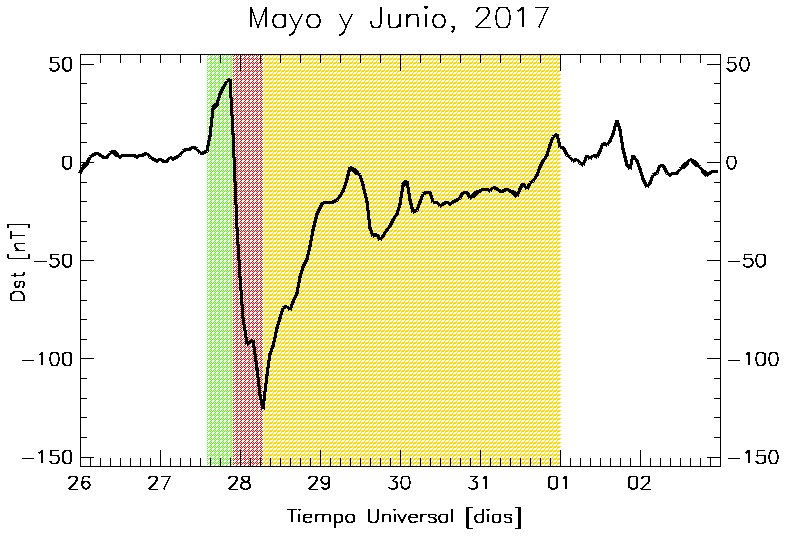
\includegraphics[width = 0.7\textwidth]{Images/dst_ex2017-05-26.png}
 	\end{center}
 	\caption{\label{tgm_ex} Ejemplo de una tormenta geomagnética acontecida a finales de mayo del 2017, cuya evolución en el tiempo es observada a través del índice geomagnético Dst. Con las regiones sombreadas se señalan las diferentes fases de la tormenta. Datos del índice Dst obtenidos de \cite{idx}} 
\end{figure}

La Figura \ref{tgm_ex} muestra un ejemplo de una tormenta geomagnética visto a través del índice Dst. En la figura se aprecian regiones sombreadas que resaltan las tres fases de una TGM: de verde el comienzo súbito, seguido por la fase principal (zona roja) y finalmente la zona amarilla sombrea a la fase de recuperación. La fase principal es un rápido decremento (valores negativos) en la intensidad de la componente horizontal a bajas latitudes del CTM. Esta etapa temporalmente coincide con la reconexión magnética entre el CMI y el CMT. La duración de esta fase principal está determinada por las condiciones del CMI y puede durar desde minutos, hasta horas \cite{l_handbook_geof_sw_Geom_field}. Al terminar la reconexión magnética la taza de inyección de partículas provenientes del VS cesa, iniciado la fase de recuperación (región de color amarillo en la figura). Durante esta fase, en ausencia del flujo de partículas anómalas, la corriente del anillo tiende a perder el exceso de partículas cargadas debido a la recombinación y la dispersión por ángulo de paso. Esto provoca un retorno gradual de la corriente del anillo a su estado pre-tormenta, lo cual provoca un debilitamiento gradual en el campo magnético inducido que se oponía al CMT. Este proceso provoca una recuperación gradual en la magnitud del CMT para eventualmente recuperar su valor pre-tormenta. Esta fase puede durar desde horas hasta varios días, dependiendo de la intensidad de la misma TGM y de las condiciones del CMI.
\vspace{ 1 em}

En ocasiones se puede presentar una fase conocida como \emph{comienzo súbito}, señalada por la región de color verde en la Figura \ref{tgm_ex}. Esta ocurre cuando, al llegar un fenómeno desencadenante (generalmente una EMC), este viene precedido por una onda de choque o región de alta presión. Cuando una onda de choque impacta a la magnetopausa, genera un efecto compresivo sobre toda la magnetosfera terrestre. Esta compresión produce una rápida intensificación del campo magnético a nivel planetario, intensificación que se percibe como un incremento en la intensidad de la componente horizontal del CMT. El comienzo súbito tiene puede durar minutos o pocas horas \cite{l_handbook_geof_sw_Geom_field} y termina al iniciar la fase principal de la tormenta (reconexión magnética).
\vspace{1 em}

\subsection{Índices geomagnéticos Dst $\Delta {\rm H}$ y SYM-H}
El índice Dst es un índice global y es el más ampliamente usado para medir la actividad magnética en latitudes bajas. Se trata de la magnitud normalizada de la componente horizontal del campo Dst (axially symmetric disturbance), como se determina de los datos de 4 observatorios de latitud baja distribuidos longitudinalmente \cite{l_handbook_geof_sw_Geom_field}. Este índice es pensado como una medida de la actividad en la corriente del anillo en tiempos de TG \cite{gombosi_1998}. Su registro es medido cada hora. Los días quietos de cada año son utilizados para establecer un promedio mínimo de la actividad en esta corriente, así como del campo magnético de fondo. Esto se resta de los registros por lo que solo las perturbaciones de esta línea base son registrados. El promedio a nivel mundial es usado a partir de 4 estaciones \cite{hargreaves_1992}. Consecuentemente, con este índice se pueden medir los cambios asociados a la intensificación en la corriente del anillo en tiempos de TG.
\vspace{1 em}

Por otro lado, con el índice $\mathrm{\Delta H}$ se determinan las condiciones del \emph{CTM} en su componente H para una escala regional. Los valores de este índice se derivan entonces, a partir de estaciones magnéticas localizadas dentro del área de estudio de interés \cite{l_handbook_geof_sw_Geom_field}. Como cada estación proporciona valores del \emph{CTM} locales, de cada estación se derivará un índice $\mathrm{\Delta H}$ distinto. Al igual que con el índice Dst, las TG generan valores negativos de campo magnético, por lo que cuanto más intensa sea una tormenta, más negativos serán los valores determinados por este índice.
\vspace{1 em}



%\subsubsection{Índice geomagnético SYM-H}
De forma adicional, a escala planetaria también se utiliza el índice SYM-H. Este índice tiene como propósito el de describir perturbaciones geomagnéticas, siendo a latitudes medias el rango en el que tiene mayor confiabilidad, en términos de perturbaciones simétricas para la componente H del \emph{CTM}. Para fines prácticos, el índice SYM-H es el equivalente del índice que Dst, pero con una cadencia de minutos en lugar de horas. \cite{idx}.\\
\vspace{1 em}

\subsection{Índice geomagnético K}

El índice K indica la intensidad de las variaciones relacionadas con perturbaciones geomagnéticas, incluyendo los efectos de impulso, pero excluyendo efectos de recuperación \cite{BARTELS_kp}. La información del índice es condensada en una escala cuasi-logarítmica, válida para estaciones en latitud geomagnética media, en el rango de los $50^\circ$. Cada estación debe elaborar su propia tabla para asignar valores de K a partir de los límites de saturación que pueden indicarse con el límite inferior para K=9. 
\vspace{1 em}

El índice K planetario (o \emph{Kp}) por otro lado, indica la intensidad de la actividad geomagnética en intervalos de tres horas, siendo un promedio estandarizado de los índices K de 12 observatorios seleccionados. Una estación estándar de esas cuenta con 500 nT como límite inferior de K=9.

\section{Manifestaciones regionales}

Mientras que las TG son fenómenos de escala global, pueden presentarse diferentes variaciones a escala regional de sus efectos. Estas variaciones pueden atribuirse a la heterogeneidad del sistema terrestre, la asimetría de sistemas de corrientes magnetosféricos e ionosféricos, así como a las interacciones entre la magnetosfera y la ionosfera en cada región. Consecuentemente, la latitud geomagnética, el tiempo local y las variaciones estacionales pueden influir en el desarrollo de una TG a nivel regional. No considerar estos factores puede conducir a incertidumbres y malinterpretaciones al intentar comprender los potenciales efectos de las TG\cite{gic_intro, gic, gic_2, gic_brazil}.  
\vspace{1 em}

La latitud geomagnética es un factor que debe tomarse en cuenta en el estudio del clima espacial regional. A mayor altitud, los efectos relacionados con las TG son más intensos. Es por ello que durante mucho tiempo, los estudios enfocados en regiones de latitudes geomagnéticas altas ($\ge 50^{\circ}$), pasando por alto regiones en latitudes medias y bajas.
\vspace{1 em}

Sin embargo, en décadas recientes, ha habido un creciente interés en estudiar los fenómenos asociados al clima espacial en regiones de latitudes medias y bajas. Se puede resaltar estudios de \cite{gic_czech, gic_brazil}, y \cite{gic}, los cuales se enfocan en investigar estos fenómenos en latitudes medias y bajas. En el caso de México, un país situado dentro de los rangos latitudinales ya mencionados, se ha echo un esfuerzo para realizar estudios magnéticos e ionosféricos \cite{MEXART2003, MEXART2005, lenica, MEXART_iono_dist, MEXART_iono_dist2, mario_rodriguez2011, lopez-montes, mario_rodriguez2014, iono-resp2016}. 

\subsection{Influencia de la Ionosfera}
\label{diono}

Se ha identificado el rol potencial de las perturbaciones ionosféricas en la inducción de respuesta geomagnética regional durante periodos de tormenta \cite[see][]{esmeralda, dramaria_1, dramaria7, P-corona1, P-corona2}. Esto es consistente con otros estudios realizados para regiones de latitud media-baja, donde se han descubierto y estudiado dos fuentes principales de variaciones geomagnéticas. Estas son las corrientes ionosféricas de dinamo perturbado o \emph{Ddyn} (por sus siglas en ingles) \cite{blanc_ddyn} y la corriente de perturbación polar número 2 o \emph{DP2} (por sus siglas en ingles) \cite{nishida_68_coherence, nishida_68_fluctuations, nishida_66_knee}.
\vspace{1 em}

Por un lado, \emph{DP2} se relaciona directamente con los campos eléctricos inducidos durante la reconexión magnética. Como se observa en la Figura \ref{fig:dp2_diag}, éstos campos eléctricos son transportados a lo largo de las corrientes de Birkeland \cite{dp2PPEF, dp2_diag}, eventualmente alcanzan la ionosfera en latitudes altas en donde inducen un par de celdas convectivas las cuales se les conoce como de perturbación polar. Las partículas cargadas en la zona entonces comienzan a tener movimiento de deriva por efectos de fuerza centrífuga y de curvatura, lo que resulta en la inducción de un campo eléctrico polarizado \cite{Hepner_a, Hepner_b, Pudovkin, blanc_caudal, Denisenko}. Durante la fase principal de la TG, éstos campos eléctricos, a la par de la corriente \emph{DP2}, pueden extenderse mas allá de las latitudes altas, cubriendo incluso latitudes bajas\cite{nishida_66_knee, nishida_68_coherence, nishida_andobayashi_67}.
\vspace{1 em}

\begin{figure}
	\centering
	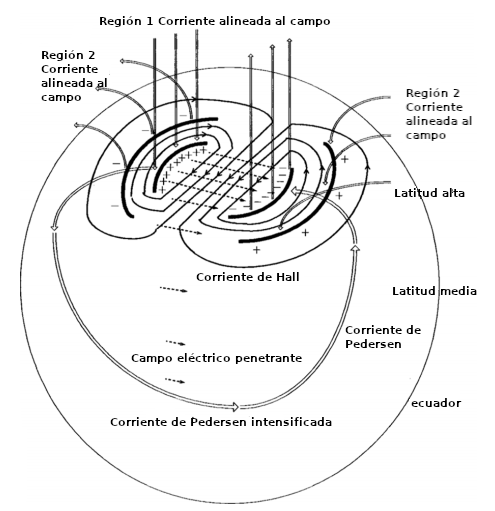
\includegraphics[width=0.5\textwidth]{Images/dp2_edited.png}
	\caption{Representación de la corriente ionosférica $DP2$ teorizada a partir de observaciones \textit{in-situ} realizadas por \cite{nishida_68_fluctuations, nishida_andobayashi_67,nishida_68_coherence}. Las corrientes ionosféricas \emph{DP2}, se componen por un par de corrientes de Hall en latitudes altas y una corriente de Pedersen que fluye en la ionosfera ecuatorial. Figura adaptada de \cite{dp2_diag}.}
	\label{fig:dp2_diag}
\end{figure}


Por otro lado, las \emph{Ddyn} representan amplificaciones de la termósfera polar debido a la precipitación de partículas energéticas durante la fase principal. En la Figura \ref{fig:ddyn_diag}, se observa que el calentamiento de Joule resultante provoca que la termosfera se expanda y tenga  flujos de circulación de viento neutro y partículas cargadas con dirección hacia el ecuador. La fuerza de coriolis induce un cambio de dirección hacia el oeste de estos flujos en latitudes bajas y medias \cite{blanc_ddyn, ddyn2005, angeoddyn}. Como consecuencia, se inducen corrientes de Pedersen y, debido a la acumulación de cargas a lo largo del ecuador magnético en el lado día se terminan generando  campos eléctricos con dirección polar y que se oponen a las primeras corrientes de Pedersen. Finalmente aparecen corrientes de Hall con dirección este, en latitudes medias ($\sim 45^\circ$), las cuales son interrumpidas en los  terminadores\cite{blanc_ddyn}. Esta secuencia de eventos resulta en corrientes divergiendo y cerrándose en latitudes adyacentes, formando un par de corrientes con forma de vórtice, conocidas como dinamo perturbado.
\vspace{1 em}

\begin{figure}
	\centering
	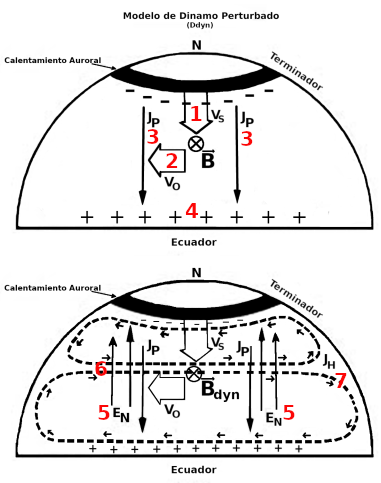
\includegraphics[width=0.5\textwidth]{Images/ddyn_diagedited.png}
	\caption{Representación gráfica del modelo del dínamo ionosférico perturbado ($ddyn$) teorizado y predicho por M. Blanch en 1980. Figura adaptada de \cite{diagrama_ddyn}.}
	\label{fig:ddyn_diag}
\end{figure}

Considerando que \emph{Ddyn} y \emph{DP2} poseen el potencial de influir en la respuesta geomagnética en latitudes medias y bajas, lleva a la pregunta si éstos son los mecanismos responsables de las variaciones locales del CMT encima de México. Previamente, \cite{tesis_yo}, estudió los efectos de estas dos corrientes en los registros magnéticos asociados con la presencia de las corrientes ionosféricas $Ddyn$ y $DP2$. En este estudio se encontró que, en general la presencia de $Ddyn$ y $DP2$ sí afectaban el campo magnético local, ocasionando variaciones de naturaleza cuasi-periódica en el mismo. Sin embargo, el número de eventos analizados fue reducido debido a los parámetros considerados para la selección de eventos, así como la disponibilidad y calidad de los datos de campo magnético locales. Lo anterior llevó también a determinadas limitaciones tanto en los datos como en el procedimiento y en el análisis de los resultados. Por ello, se requiere incrementar el estudio precedente a través del análisis de una base de datos mayor. De igual forma, se puede realizar un fortalecimiento de los resultados a través de implementar herramientas de análisis adicionales y mejorar las ya implementadas.








\section{Procesamiento de datos magnéticos}

Para poder realizar estudios de TG para regiones específicas, se utilizan los registros de magnetómetros posicionados en esa región de interés. A partir de las observaciones de estos magnetómetros como tal, se busca obtener información sobre las variaciones de las corrientes eléctricas en ionosfera y magnetósfera \cite{BARTELS_kp}. Sin embargo, éstas observaciones directas también reciben información de otras fuentes de campo magnético que no son de interés para este tipo de estudios \cite{amorymazaudier_2017, amory2020_filtros}. Por lo tanto, el pre-procesado y procesado de los datos de salida del magnetómetro se vuelve una parte imprescindible.
\vspace{1 em}

\subsection{Derivación de lineas base}

El \emph{CMT} presenta variaciones a diversas escalas de tiempo, variaciones que implican transferencia de energía hacia o desde el mismo \emph{CMT} \cite{l_handbook_geof_sw_Geom_field}. Las fuentes principales que contribuyen a los cambios significativos en el \emph{CMT} total son:
\begin{itemize}
    \item los procesos convectivos en el núcleo terrestre;
    \item la magnetización remanente de la corteza terrestre;
    \item la radiación solar electromagnética;
    \item la interacción con el viento solar; y
    \item las corrientes ionosféricas y magnetosféricas
    \item los efectos de marea sobre la ionosfera.    
\end{itemize}

La primer fuente descrita, constituye lo que se conoce como campo magnético estable, cuyos cambios se presentan en periodos de decenas, cientos o miles de años \cite{l_handbook_geof_sw_Geom_field}. El campo resultante es, para fines prácticos, un dipolo casi centrado con el centro de la Tierra \cite{hargreaves_1992}, con una desviación entre los polos magnéticos y el eje de rotación terrestre de aproximadamente $11.5^\circ$. Su magnitud aproximada a nivel de superficie y en el ecuador magnético es de $\sim 3.1 \times 10^{5}$ nT \cite{l_handbook_geof_sw_Geom_field, l_basic_spaceplasmaphysic, l_russell}. Su interacción con el VS da lugar a la cavidad magnética conocida como magnetosfera.\\
\vspace{1 em}

A partir del ``campo estable'', se pueden identificar o definir variaciones para diferentes escalas de tiempo. Por una parte están aquellas variaciones cuyos cambios se miden en años o variación \emph{secular} \cite{l_handbook_geof_sw_Geom_field}. Por otro lado, el \emph{CMT} muestra variaciones cíclicas con periodos menores al año, variaciones conocidas como \emph{variaciones quietas} \cite{l_handbook_geof_sw_Geom_field}. Estas variaciones son ocasionadas por los efectos de radiación electromagnética proveniente del Sol, que resultan directamente con la variación diurna. También se presentan variaciones magnéticas debido a los efectos gravitacionales de marea ocasionados por el Sol y la Luna sobre la ionosfera \cite{BARTELS_kp}.
\vspace{1 em}

Los efectos de la radiación solar también se conocen como \emph{variación de Sol Quieto} o ($H_{SQ}$). Tiene como origen el calentamiento y a la ionización que la radiación solar genera sobre la ionosfera terrestre. El proceso provoca la aparición de corrientes de viento neutro, arrastrando partículas ionizadas en la atmósfera de la Tierra; las corrientes inducen campos magnéticos que afectan regional y temporalmente al \emph{CMT}. Estas variaciones tienen amplitudes en el rango de $10-100$ nT a lo largo del día \cite{iaga_guide, baseline_Gjerloev}. La intensidad de éstas fluctuaciones dependen de factores como la latitud geomagnética, la temporada del año, la hora local, e incluso, de la intensidad de la radiación solar debido a la actividad del Sol \cite{iaga_guide, gombosi_1998, l_handbook_geof_sw_Geom_field}.\\
\vspace{1 em}

En el caso de los efectos de marea, éstos se relacionan con un tipo de variación que se conoce como variación día a día. Esta variación consiste en que de un día a otro habrán cambios en el comportamiento de la variación diurna. Como resultado, se obtendrían cambios en la magnitud máxima de un día a otro. Según \cite{iaga_guide}, las variaciones día a día o $H_0$, tienen pequeñas amplitudes, de apenas $\sim 10$ nT, aunque su intensidad también depende de factores como la actividad solar, la estacionalidad, la rotación solar, entre otros mencionados previamente. 
\vspace{1 em}

Son éstas dos las variaciones regulares aquellas de mayor interés para ventanas de tiempo que involucren el estudio de una TG, es necesario poder identificarlas en los registros magnéticos y remover sus efectos, para quedarnos únicamente con la contribución magnética asociada a la TG. De esta forma, también se remueve el efecto del CMT principal de la Tierra (del orden de $\sim 30 000$ nT). A continuación se describirá de forma breve este proceso.

\subsubsection{Linea base día a día}
Según \cite{baseline_Gjerloev}, es posible determinar la línea base día a día. Para ello, el primer paso es identificar el valor típico diario: Este puede ser el promedio o la mediana de los datos para cada día. No obstante, el criterio del qué considerar como valor típico diario depende del autor. Por ejemplo, \cite{vanKampt} considera como valor típico la mediana de los datos al medio día, mientras que \cite{ionos1} considera como linea base un promedio de los 5 días más quietos. En el caso del trabajo de \cite{2021amory}, aquí se considera como valor típico al promedio de los datos durante media noche, para aquellos días quietos. Por otro lado, \cite{baseline_Gjerloev} en vez de utilizar un promedio o una mediana, hace uso de un ajuste Gaussiano. Finalmente, para este trabajo, inicialmente se consideró como valor típico diario la mediana de todo el día para cada día. 
\vspace{1 em}

Una vez que se obtiene el valor típico para cada día, estos valores se deben interpolar, generando una serie de tiempo con resolución de 1 minuto (la resolución debe ser la misma que la de los datos originales). Una vez que se derive esta linea (que denominamos como $H_0$), simplemente se resta de la serie $H$. En la Figura \ref{fig:diadia1} se muestra paso a paso la realización del procedimiento de derivación de la linea base $H_0$ a partir de los datos de salida.
\vspace{1 em}

\begin{figure*}[h!]
    \centering
    \centerline{\Large \bf   
      %\hspace{0.18\textwidth}  \color{black}{\Large{Res}}
       %\hspace{0.28\textwidth}  \color{black}{\Large{Res+TC}}
         \hfill}
          \centerline{\Large \bf   
         \hfill}
     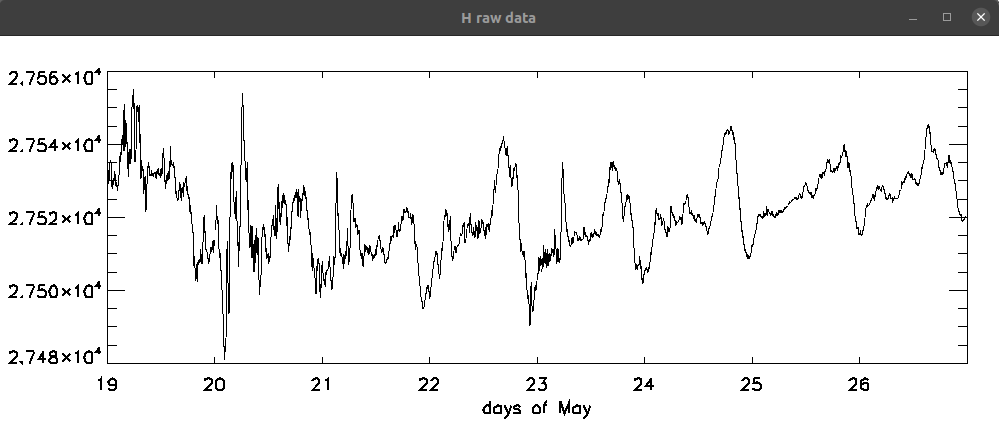
\includegraphics[width=10.0cm]{Images/cap2/lineabase/diadia/paso1.1.png}
     \centerline{\Large \bf   
         \hfill}
     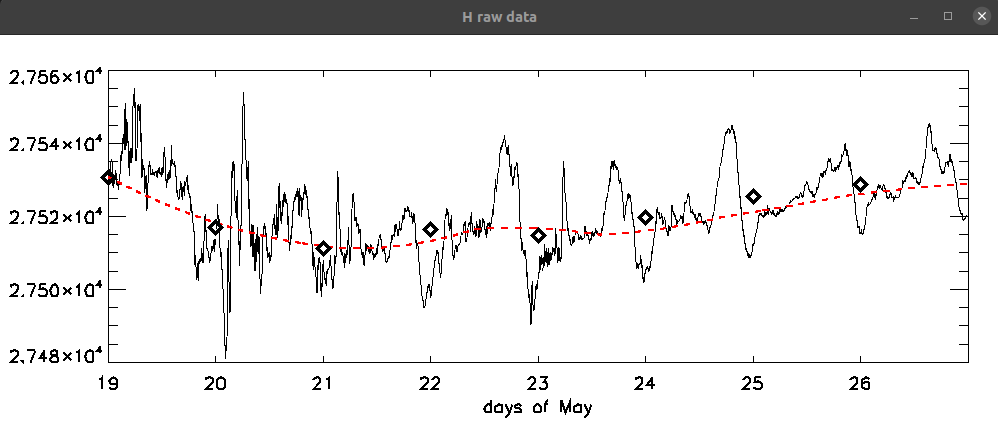
\includegraphics[width=10.0cm]{Images/cap2/lineabase/diadia/paso1.2.png}     
     \centerline{\Large \bf   
         \hfill}
      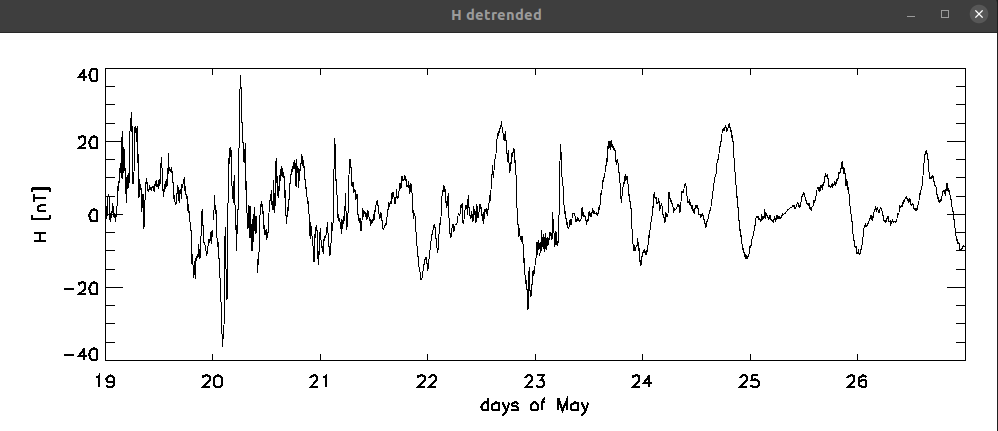
\includegraphics[width=10.0cm]{Images/cap2/lineabase/diadia/paso1.3.png}         
       \caption{Datos de salida de campo magnético, proporcionados por TEO(arriba), los rombos abiertos señalan los valores típicos (en medio) y su interpolación (linea roja) que será la linea base $H_0$. Los efectos removidos se muestran en el panel inferior.}
    \label{fig:diadia1}
\end{figure*}

No obstante, existe un problema al momento de llevar a cabo este procedimiento en ventanas de tiempo que enmarquen una TG. El punto clave en este caso, es que los días de tormenta, como su nombre lo indica, no manejan valores típicos, sino que son valores de perturbados a extremos. Estos valores no típicos, terminan influyendo en la serie de tiempo calculada, deformándola tal y como se observa en el panel inferior de la Figura \ref{fig:diadia2}, específicamente los días 28 y 29 de mayo que corresponden a días de tormenta. 
\vspace{1 em}

\begin{figure*}[h!]
    \centering
    \centerline{\Large \bf   
      %\hspace{0.18\textwidth}  \color{black}{\Large{Res}}
       %\hspace{0.28\textwidth}  \color{black}{\Large{Res+TC}}
         \hfill}
          \centerline{\Large \bf   
         \hfill}
     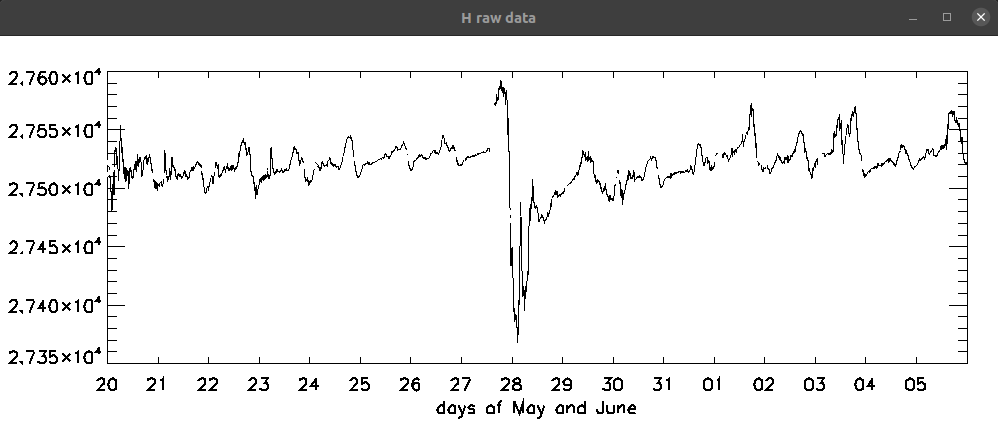
\includegraphics[width=10.0cm]{Images/cap2/lineabase/diadia/paso2.1.png}
     \centerline{\Large \bf   
         \hfill}
     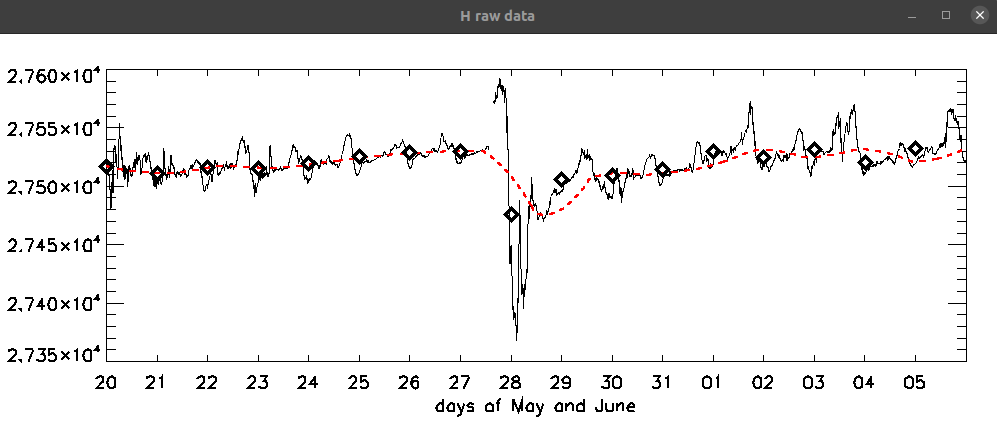
\includegraphics[width=10.0cm]{Images/cap2/lineabase/diadia/paso2.2.png}     
     \centerline{\Large \bf   
         \hfill}
      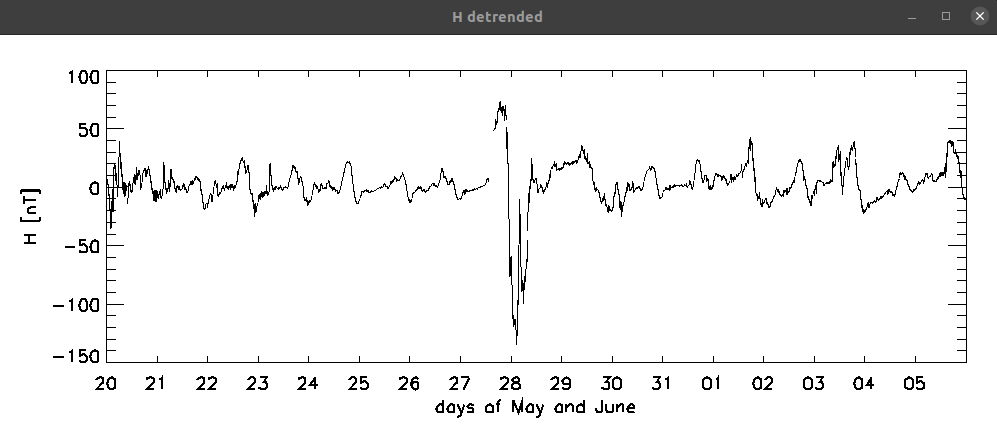
\includegraphics[width=10.0cm]{Images/cap2/lineabase/diadia/paso2.3.png}         
       \caption{Datos de salida de campo magnético para un evento de tormenta, proporcionados por TEO(arriba), los rombos abiertos señalan los valores típicos (en medio) y su interpolación (linea roja segmentada) que será la linea base $H_0$. Los efectos removidos se muestran en el panel inferior.}
    \label{fig:diadia2}
\end{figure*}

Para poder solucionar este problema, Es necesario considerar un umbral con el cual, el algoritmo de pre-procesamiento utilizado detecte los valores diarios asociados a periodos de tormenta. Así, todo valor que sobrepase el umbral será considerado como un día perturbado:
\begin{equation}
    \begin{split}
        LIM_{sup} = \Bar{H} + n \cdot \sigma \\
        LIM_{inf} = \Bar{H} - n \cdot \sigma,
    \end{split}    
\end{equation}
donde \emph{n} es un cualquier factor que se ajuste al caso de estudio (n=1.5 suele ser un buen valor para comenzar \cite{Dealing_with_outliers}) y $\Bar{H}$ es el promedio de la serie de tiempo que, en este caso, se trata de la componente horizontal del CMT local. \cite{baseline_Gjerloev, vanKampt} utilizan este criterio para los valores diarios de resolución 24h. Todo valor que se encuentre por fuera de este rango será considerado como valor nulo (NaN) y reemplazado usando una interpolación con los valores vecinos. En este trabajo, se consideró usar el criterio utilizado por \cite{phdthesis_ramon}, donde en vez de utilizar el promedio y la desviación estándar, se utilizan los cuartiles:

\begin{figure*}[h!]
    \centering
    \centerline{\Large \bf   
      %\hspace{0.18\textwidth}  \color{black}{\Large{Res}}
       %\hspace{0.28\textwidth}  \color{black}{\Large{Res+TC}}
         \hfill}
          \centerline{\Large \bf   
         \hfill}
     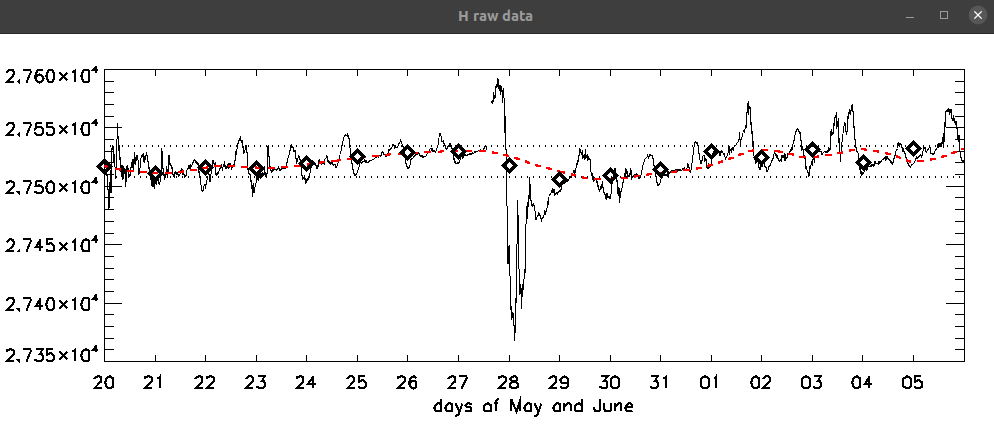
\includegraphics[width=10.0cm]{Images/cap2/lineabase/diadia/paso3.1.png}
     \centerline{\Large \bf   
         \hfill}
     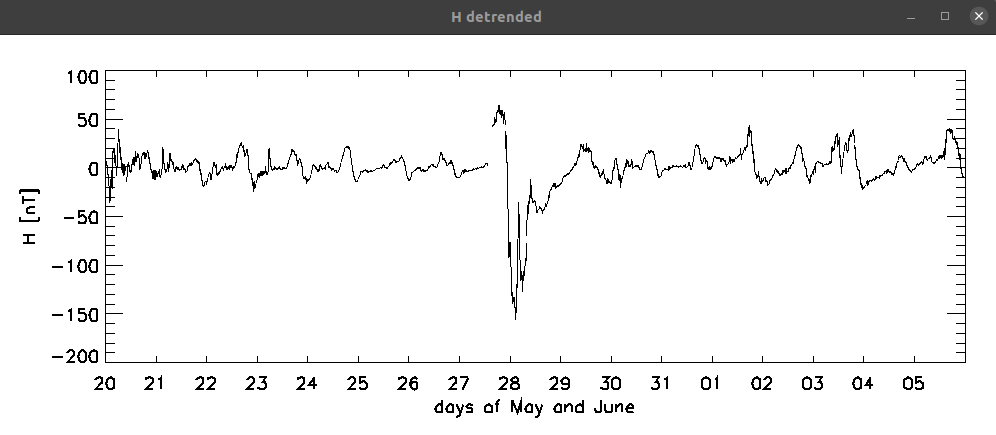
\includegraphics[width=10.0cm]{Images/cap2/lineabase/diadia/paso3.2.png}            
       \caption{Derivación corregida de la linea base $H_0$.}
    \label{fig:diadia3}
\end{figure*}


\begin{equation}
\label{eq:iqr}
    \begin{split}
        LIM_{sup} = M_{H} + n \cdot IQR \\
        LIM_{inf} = M_{H} - n \cdot IQR,
    \end{split}    
\end{equation}

La ventaja de utilizar el rango intercuartil así como la Mediana, se basa en que se tratan de valores estadísticos más robustos y menos sensibles al efecto de valores extremos que pudieran presentarse en la serie de tiempo. Gracias a este procedimiento, se podrá derivar de forma más precisa la linea base $H_0$ para periodos de tormenta. El resultado de este procedimiento se muestra en la Figura \ref{fig:diadia3}, donde ya no se observa la deformación de la serie de tiempo original, tal y como ocurre en la Figura \ref{fig:diadia2}. Cabe señalar que, de acuerdo con \cite{baseline_Gjerloev}, la cantidad de días que abarque la ventana de tiempo debe ser suficientemente grande, debido a que se derivará un dato por día. Es por ello que, para que los valores diarios tengan una significancia estadística, la ventana de tiempo debería ser de por menos 10 a 15 días, especialmente al considerar que la ventana de tiempo involucra días perturbados, los cuales serán descartados por medio del algoritmo.
\vspace{1 em}

\subsubsection{Linea base diurna}

La clave para la derivación de la línea base diurna son los días quietos. Se trata de los días oficialmente caracterizados por tener menor actividad geomagnética relacionada con la actividad solar. Para cada mes, se generan listas que contienen los datos de los diez días más quietos, tomando como referencia al índice Kp \cite{BARTELS_kp}. Cada mes, los datos son procesados en orden y promediados diariamente; los días con menor orden son los seleccionados como más quietos. La forma tradicional de derivar la linea base diurna es a través de promediar los datos magnéticos durante los cinco días más quietos. La información de los días más quietos de cada mes se encuentra en el sitio oficial del Servicio Internacional de Índices Geomagnéticos (ISGI por sus siglas en inglés), el cual proporciona la información de los días quietos derivados a partir del criterio antes mencionado.
\vspace{1 em}

Posteriormente, se genera una linea base a partir de este promedio que se denominará como $H_{SQ}$, la cual será restada de la serie de tiempo original o:
\vspace{1 em}

\begin{equation}
\label{eq:lineabase}
    H- H_0-H_{SQ}
\end{equation}

Sin embargo, una sumatoria de índices K puede llevar a un resultado engañoso ya que \textit{hay meses en que los días realmente quietos no ocurren. En estos casos, incluso aquellos 5 días seleccionados como menos perturbados presentan un nivel de perturbación tal que, en meses verdaderamente quietos, sus valores serían considerados como relativamente perturbados} \cite{BARTELS_kp}.
\vspace{1 em}

Por otro lado, existe un segundo problema que está relacionado con el objetivo de este trabajo: así como las perturbaciones geomagnéticas varían dependiendo de la región de estudio, también hay variaciones en periodos de quietud geomagnética. Mientras que para una región, puede haber un periodo de quietud geomagnética, en otra región pueden presentarse variaciones significativas, por lo que tal día ya no se consideraría quieto. Así, días considerados como quietos según el índice Kp, podrían ser no del todo quietos a escala local. Es por ello, que para considerar los días más quietos, éstos deben seleccionarse con base en datos magnéticos locales (y no planetarios, como es el caso de los días proporcionados por el ISGI). 
\vspace{1 em}

El criterio utilizado en este trabajo es el mismo seguido por \cite{baseline_Gjerloev, vanKampt}, de la máxima fluctuación diaria. Para una ventana de tiempo con suficientes días y con una resolución de 1 minuto, se hace un re-muestreo de los datos a 1h. Cada hora, se calcula la desviación estándar (como en \cite{vanKampt}) o bien, como se hizo en este caso, utilizando el rango intercuartil. Éstos valores horarios describen el grado de variación magnética, siendo el siguiente paso, seleccionar la máxima variación por cada día o el $MAX(\sigma)/MAX(IQR)$. Aquellos picos diarios de menor valor en la ventana de tiempo, serán considerados como días quietos locales o \emph{DQL}.
\vspace{1 em}

El siguiente paso es el de generar la linea base, y para ello, \cite{vanKampt} considera que no es necesario utilizar los 5 días quietos por cada mes. El motivo es que habrían meses altamente perturbados, donde los días clasificados como quietos en realidad no sean del todo ``quietos'', por lo que un promedio de éstos podría no ser la mejor opción. Esto sin mencionar que solamente 1 o dos días podrían considerarse como verdaderamente quietos. En su lugar, \cite{vanKampt} utiliza únicamente dos \emph{DQL}: un día previo al evento y el segundo posterior al evento, enmarcando a la TG. Entre más cercanos (temporalmente) sean los DQL entre sí, la linea base será más precisa, aunque el umbral de separación entre los \emph{DQL} puede ser de hasta 66 días \cite{vanKampt}.
\vspace{1 em}

A partir de aquí, \cite{vanKampt} aplica un análisis de Fourier, generando la serie de tiempo $H_{SQ}$ a base de un filtro pasa-bajas, para solo considerar las fluctuaciones asociadas a la variación diurna. Para este trabajo inicialmente se combinó con el criterio de \cite{baseline_Gjerloev} realizando una interpolaron linealmente los DQL al medio día sin aplicar previamente el filtro basa-bajas. A esta interpolación se le aplicó una función de suavizado por cada 30 minutos, siendo la serie resultante, la linea base $H_{SQ}$. En la Figura \ref{fig:diasq} se puede observar el procedimiento llevado a cabo. En el panel superior se muestra que a partir de dos DQL se generan dos series de tiempo (lineas azul y roja), haciendo la interpolación se genera la linea base $H_{SQ}$ a la cual se le aplica la función de suavizado. Posteriormente, en el panel inferior se muestra el resultado de remover este efecto descrito en la Ecuación \ref{eq:lineabase}. La linea negra representa la serie de tiempo previa a remover el efecto $H_{SQ}$, mientras que la linea roja representa la serie de tiempo, removiendo $H_{SQ}$. Se puede apreciar una atenuación de los efectos de variación diurna para cada día, sin que éste afecte a los valores durante el periodo en que ocurre la TG.
\vspace{1 em}


\begin{figure*}[h!]
    \centering
    \centerline{\Large \bf   
      %\hspace{0.18\textwidth}  \color{black}{\Large{Res}}
       %\hspace{0.28\textwidth}  \color{black}{\Large{Res+TC}}
         \hfill}
          \centerline{\Large \bf   
         \hfill}
     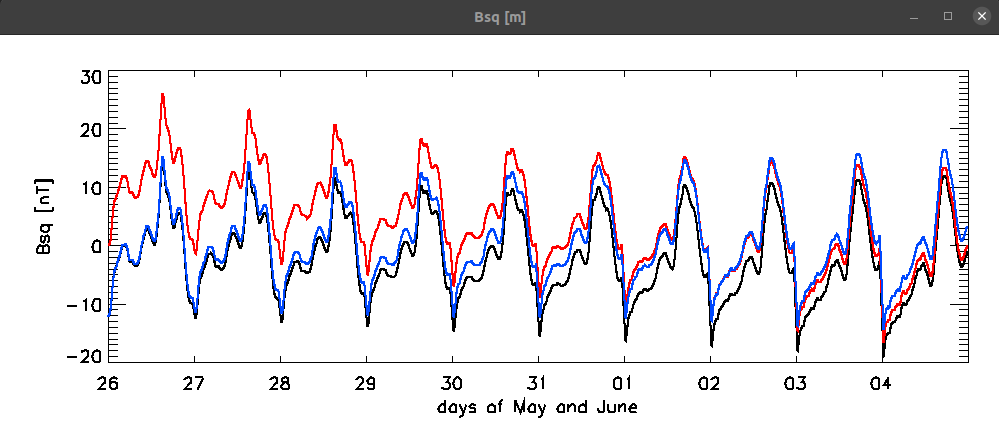
\includegraphics[width=10.0cm]{Images/cap2/lineabase/diurno/sq.png}
     \centerline{\Large \bf   
         \hfill}
     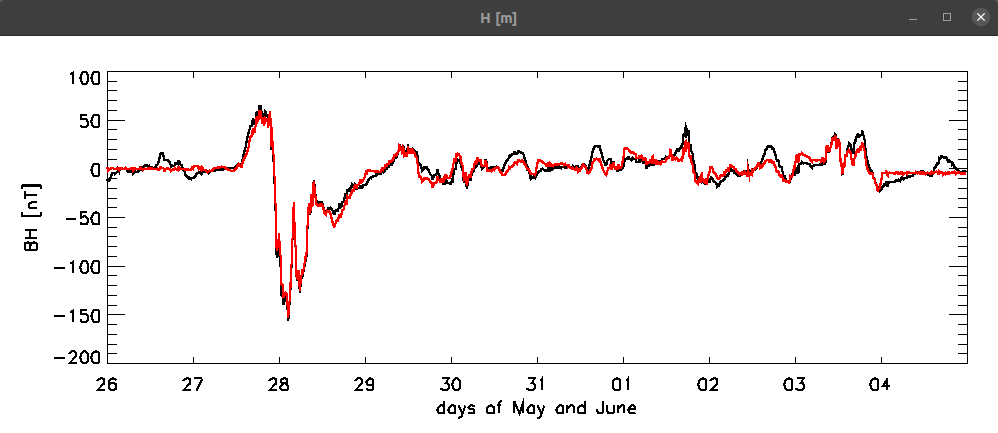
\includegraphics[width=10.0cm]{Images/cap2/lineabase/diurno/sq2.png}            
       \caption{Derivación de la linea base $H_{SQ}$.}
    \label{fig:diasq}
\end{figure*}


\subsection{valores extremos: picos de datos}
Una de las dificultades que se presentan al pre-procesar los datos de campo magnético son los valores extremos. Éstos valores pueden afectar los análisis posteriores, por lo que es sumamente importante poder generar un algoritmo que los detecte y elimine de la serie de tiempo a pre-procesar.
\vspace{1 em}

Los valores extremos en los datos son valores que se desvían de la tendencia general en las observaciones, tal y como se observa en el panel superior de la Figura \ref{fig:picos}. En general, pueden indicar una variabilidad en mediciones experimentales o tratarse de errores en las mediciones\cite{brief_overview_outlier-detection}.
\vspace{1 em}

Dependiendo del tipo de medición, los valores extremos pueden ser del tipo: puntuales, contextuales o colectivos. 

\begin{enumerate}
    \item Los valores puntuales o picos, son valores únicos cuya magnitud se aleja del resto de los datos en la distribución.
    \item Los contextuales se refieren al ruido de fondo en los datos.
    \item Los colectivos pueden tratarse de subconjuntos de novedades en los datos, como una señal que podría tratarse de un caso de interés.
\end{enumerate}

Las causas principales de estos valores extremos son:
\begin{itemize}
    \item errores en los datos de entrada (errores del operador)
    \item errores de medición (error instrumental)
    \item errores experimentales (datos de extracción o planteamiento experimental/ejecución de errores)
    \item intencional (errores aleatorios para prueba)
    \item errores de procesamiento de datos (manipulación de datos)
    \item errores de muestreo
    \item naturales (no necesariamente un error, sino un fenómeno no contemplado)
\end{itemize}

El detectar valores extremos como los picos, es de gran importancia en casi cualquier disciplina, por lo que es necesario considerar las siguientes interrogantes: ¿Cuales y cuantas características se considerarán para detectarlos?¿Se puede asumir las distribuciones de los valores para las características seleccionadas?
\vspace{1 em}

Algunos de los métodos más populares para la detección de valores extremos son:

\begin{itemize}
    \item Registro Z
    \item modelado de probabilidad y estadística
    \item modelos de regresión lineal
    \item modelos basados en proximidad
    \item modelos de información teórica
\end{itemize}

\subsubsection{Algoritmo de Whitaker-Hayes}
Se trata de un método altamente eficiente para lidiar con la detección de valores extremos únicos o picos \cite{Dealing_with_outliers}. Una ventaja que proporciona este algoritmo es que es lo suficientemente poco costoso, computacional mente hablando, como para ser ejecutado por la mayoría de sistemas computacionales \cite{WHITAKER2018}. Es necesario considerar sin embargo, que los datos deben tener una distribución cercana a la normal \cite{Dealing_with_outliers, brief_overview_outlier-detection}.
\vspace{1 em}

Éste algoritmo hace uso de una versión modificada del \emph{Puntaje Z}. Este método es un buen inicio para el tratamiento de valores extremos \cite{removing_with_Whitaker-Hayes}. Consiste en determinar qué tan alejado está un determinado valor con respecto a un promedio o mediana en la distribución de datos, usando medidas de variaciones (desviación estándar o rango intercuartil). El \emph{Puntaje Z} se calcula a partir de una serie de tiempo H de la siguiente forma:

\begin{equation}
    |z(i)| = | \frac{(H(i)-\Bar{H})}{\sigma} |
\end{equation}
Para detectar picos usando el \emph{Puntaje Z} es necesario ajustar los umbrales superiores e inferiores \cite{Dealing_with_outliers, removing_with_Whitaker-Hayes}.
\vspace{1 em}

Como mejor alternativa, uno puede hacer uso del \emph{Puntaje Z modificado} o \emph{PZM}. Éste método utiliza la desviación de la mediana absoluta (DMA), en lugar del promedio y se calcula de la siguiente forma:
\begin{equation}
    |z(i)| = | 0.6745 \cdot \frac{H(i) - M}{DMA}|,
\end{equation}
donde $DMA = |H-M|$, siendo $M$ la mediana de la serie de tiempo H(i). La ventaja es que la mediana y DMA son medidas más robustas de la tendencia central y la dispersión respectivamente. El multiplicador de 0.6745 es el cuartil 75 de la distribución normal estándar \cite{removing_with_Whitaker-Hayes}.

Para poder lidiar con los picos \cite{WHITAKER2018, removing_with_Whitaker-Hayes} consideran sus características de tener una alta diferencia con respecto de sus valores vecinos, así como un efecto de aumento agudo (no gradual). De esta forma, consideran que usando una derivada de primer orden en los datos consecutivos o $\nabla H(i) = H(i)- H(i-1)$ para calcular el PZM. Se observará un efecto de aplanamiento sobre las variaciones graduales, mientras que los picos que son delgados y de incremento agudo, son preservados, tal y como se aprecia en el panel de en medio de la Figura \ref{fig:picos}. Así, el algoritmo se expresa de la siguiente forma:
\begin{equation}
    |z(i)| = | 0.6745 \cdot \frac{\nabla H(i) - M}{MDA}|
\end{equation}

el criterio propuesto por la \emph{Sociedad Americana de Control de Calidad} es a partir de 3.5 , aunque de acuerdo con \cite{removing_with_Whitaker-Hayes}, el umbral dependerá de la serie de tiempo. El paso final es reemplazar por valores nulos y, en caso de ser necesario, es posible reemplazarlos a partir de una interpolación con los valores vecinos, tal y como se muestra en la Figura \ref{fig:picos}.

\begin{figure*}[h!]
    \centering
    \centerline{\Large \bf   
      %\hspace{0.18\textwidth}  \color{black}{\Large{Res}}
       %\hspace{0.28\textwidth}  \color{black}{\Large{Res+TC}}
         \hfill}
          \centerline{\Large \bf   
         \hfill}
     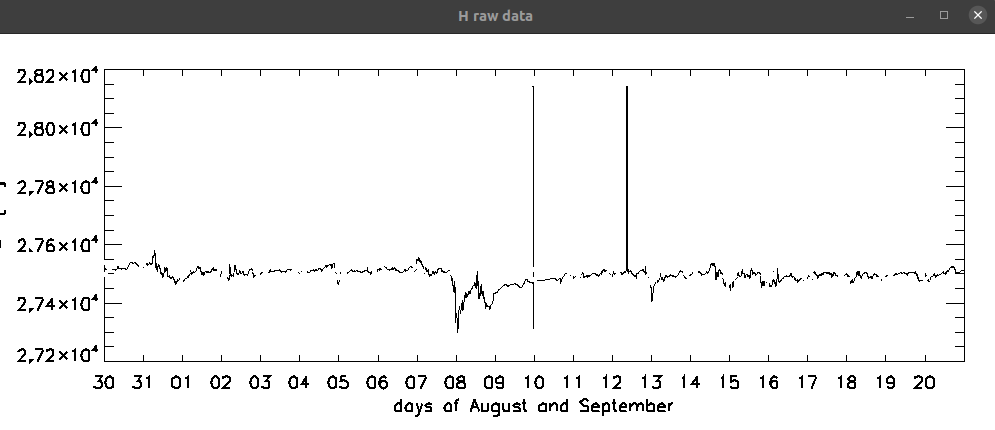
\includegraphics[width=10.0cm]{Images/cap2/lineabase/picos/picos.png}
     \centerline{\Large \bf   
         \hfill}
     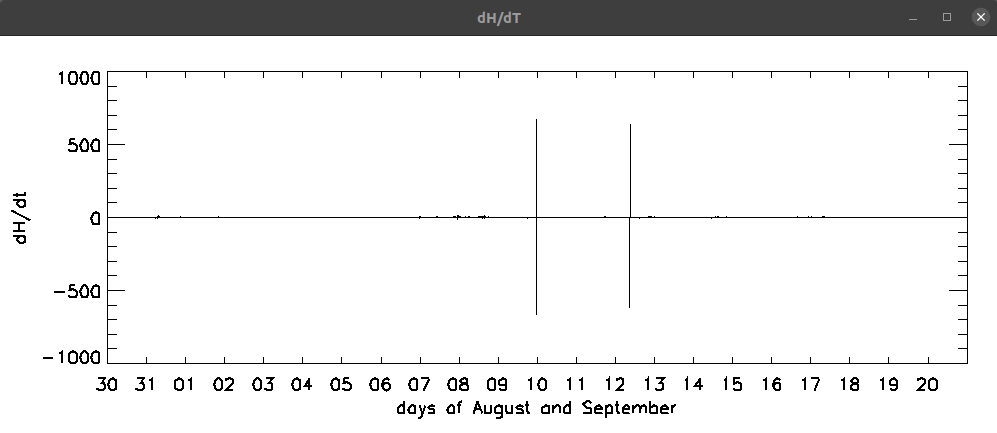
\includegraphics[width=10.0cm]{Images/cap2/lineabase/picos/picos2.png}     
     \centerline{\Large \bf   
         \hfill}
      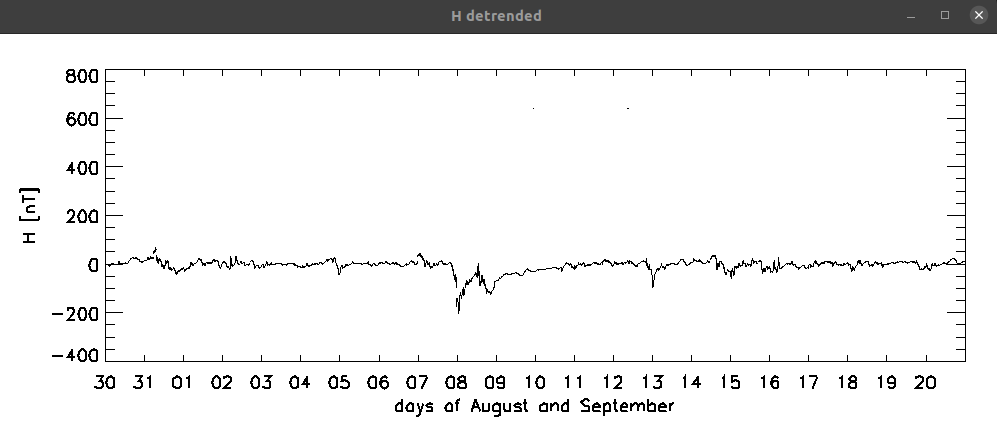
\includegraphics[width=10.0cm]{Images/cap2/lineabase/picos/picos3.png}         
       \caption{Datos de salida de campo magnético para un evento de tormenta, proporcionados por TEO(arriba), los rombos abiertos señalan los valores típicos (en medio) y su interpolación (linea roja) que será la linea base $H_0$. Los efectos removidos se muestran en el panel inferior.}
    \label{fig:picos}
\end{figure*}

\section{Análisis de Señales}

\subsection{Teorema de Percival y el Espectro de potencia}
\label{psd_section}
De acuerdo con el teorema de Percival, la energía de la señal se relaciona con la contribución de la densidad de energía en el sistema, a partir del parámetro a medir \cite{book_analysis_Method_multiSp_data}. La relación de Percival se describe por medio de la siguiente expresión: 

\begin{equation}
    \frac{1}{T} \int_{t0}^{t0+T} H^2(t)dt = \Tilde{H}[0] + 2 \sum_{n=1}^\infty |\Tilde{H}[n]^2|
\end{equation}

Los términos de la ecuación dependen de la longitud del intervalo T. Mientras que el lado izquierdo de la ecuación permanece igual (al modificar T), el lado derecho tendrá un cambio en el espaciamiento de las frecuencias $\Delta f = 1/T$. Entonces, los coeficientes en $|\Tilde{H}[n]|$ dependen de la longitud de la señal. Para poder describir entonces la distribución de la densidad de la energía de la señal en el espacio de frecuencias, introducimos la función \emph{PSD}:

\begin{equation}
    PSD[n] = 2T |\Tilde{H}|^2
\end{equation}

para todo $n$ positivo. Entonces, la relación de Percival toma la forma de:

\begin{equation}
    \frac{1}{T} \int_0^T H^2 (t)dt = PSD[0] \frac{\Delta f}{2} +2 \sum_{n=1}^\infty PSD[n] \Delta f
\end{equation}

Habiendo definido \emph{PSD}, su valor para una frecuencia en particular no cambiará con distintos T. La \emph{PSD} tiene una interpretación física inmediata: se trata de la contribución de la energía de la señal a partir de cada intervalo de frecuencia $\Delta f$ alrededor de $f_n$. Esto solo puede ser usado para frecuencias reales, ya que ignora las del conjunto imaginario.
\vspace{1 em}

La otra parte de la señal se encuentra en el espectro de fase, definido como:
\begin{equation}
    \Tilde{H}[n] = |\Tilde{H}[n]| exp(i\varphi [n]), 
\end{equation}

donde $\varphi [-n] = -\varphi[m]$ y $\varphi[0]=0$. el valor absoluto de la fase depende de la posición inicial del muestreo de la señal.
\vspace{1 em}

\subsubsection{Función Ventana}

Considerando que, tanto la transformada discreta de Fourier como PSD consideran las series de tiempo como infinitas, al usar series de tiempo de duración finita conduce a un problema: el efecto de borde. La abrupta interrupción en una ventana de tiempo usada (denominada como rectangular) ocasiona una pérdida de energía desde cualquiera de los picos espectrales, hacia las frecuencias vecinas. Esto se debe a que el efecto escalón debido al borde provoca una dispersión en la energía, la cual es transferida \cite{book_analysis_Method_multiSp_data}.
\vspace{1 em}

Como solución para este fenómeno, se han diseñado una gran variedad de funciones ventana. Se trata de un subconjunto de la serie de tiempo (o sub-ventanas de la ventana original) a la cual se le aplica una función, la cual se irá recorriendo para toda la serie de tiempo. Como tal, las funciones ventanas no pueden llevar la pérdida de frecuencia a cero, sin embargo tienen la capacidad de atenuar la pérdida de energía que normalmente se dispersa hacia las demás frecuencias, ocasionando un incremento en el grosor del pico principal.
\vspace{1 em}

En este punto, es importante dedicar esfuerzo a la selección de parámetros de la ventana (y a la selección de la función ventana). No obstante, el objetivo principal es \textbf{no usar una ventana rectangular}.
\vspace{1 em}

En general, al multiplicar la señal por coeficientes de las ventanas (que suelen ser menores a 1), se obtiene una pérdida general de la energía. Esta pérdida depende de la señal en sí, pero al considerar la relación de Percival, se tiene que el decremento estadístico esperado de los valores del PSD debido a la función ventana es del promedio del cuadrado de la ventana:

\begin{equation}
    W_{pc} = \frac{1}{N} \sum_{j=0}^{N-1} w[j]^2,
\end{equation}

por lo que para compensar la pérdida de energía en el PSD, posterior a la aplicación de la función ventana, el PSD debe dividirse por $W_{pc}$.
\vspace{1 em}

\subsection{Análisis de Ondículas}

La técnica para representar variaciones rápidas en el dominio de la frecuencia y variaciones lentas en el dominio del tiempo se conoce como análisis tiempo-frecuencia. La relación entre tiempo-frecuencia (alta-baja resolución) depende de las propiedades de la señal, para saber si se quiere que el tiempo tenga mayor resolución, a expensas de resolución en frecuencia o viceversa \cite{book_analysis_Method_multiSp_data}. La aplicación de este tipo de análisis tiene ciertas ventajas, ya que permite detectar el momento en el tiempo en que se presentan ciertas fluctuaciones a determinada frecuencia. Esto es algo que no puede observarse en los espectros de potencia, donde sólo se muestran los picos de potencia, pero no se muestra el tiempo en que se presentan (bien puede tratarse de un efecto limitado a un corto periodo, o un efecto persistente). Esta es la idea del uso de las ondículas, pues el poder localizar en tiempo determinadas fluctuaciones a ciertas frecuencias o trenes de ondas implica una ventaja al no saber si se trata de una señal persistente o muy breve en la ventana. 
\vspace{1 em}

La transformada Wavelet o de ondícula puede ser utilizada para analizar series de tiempo que contengan una potencia no estacionaria en diferentes frecuencias \cite{guide_wavelet_routines}. De la misma forma, es necesario considerar la forma o función de la ondícula $\psi_0(n)$ donde $n$ es un parámetro de tiempo. Una función ondícula, como la ondícula Morlet tiene la siguiente forma:

\begin{equation}
    \psi_0(n) = \pi^{1/4}e^{i \omega_0 n} e ^{-n^2/2}
\end{equation}

donde $\omega_0$ es una frecuencia adimensional. El término función wavelet o de ondícula se refiere a ondículas ortogonales o no ortogonales. Para series de tiempo discretas, se utiliza una transformada discreta que tiene la siguiente forma: 

\begin{equation}
    W_n(s) = \sum_{k = 0}^{N-1} \hat{x}_k \hat{\psi} \ast (s \omega_k) e^{i \omega_k n {\displaystyle \delta} t}
\end{equation}

donde $\hat{x}_n$ es una transformada discreta de Fourier, $k=0...N-1$ es el índice de las frecuencias, $s$ es la escala que permite modificar la amplitud de la forma sinusoidal resultante y la frecuencia angulas $\omega_k$ se define como:

\begin{equation}
    \begin{split}
        \omega_k = \frac{2 \pi k}{N {\displaystyle \delta} t} : k \le \frac{N}{2}\\
        \omega_k = - \frac{2 \pi k}{N {\displaystyle \delta} t} : k > \frac{N}{2}
    \end{split}
\end{equation}

Una practica común \cite{book_analysis_Method_multiSp_data, guide_wavelet_routines} es la de normalizar las transformadas de ondícula, para que puedan compararse unas con otras, mediante la siguiente expresión:

\begin{equation}
    \hat{\psi}(s \omega_k) = (\frac{2 \pi s}{{\displaystyle \delta} t} )^{1/2} \hat{\psi}_0 (s \omega_k)
\end{equation}

Por otro lado, así como es posible obtener la energía de la señal derivada a partir del teorema de Percival, también es posible hacer lo propio con la transformada de ondícula, siendo ésta la potencia espectral de la ondícula definida como $|W_n(s)|^2$. Al igual que con los \emph{PSD}, la potencia de la ondícula permite visualizar los picos de energía de las frecuencias más significativas, con la diferencia en que también se obtiene información en el dominio del tiempo.

\chapter{Trabajo de investigación: Efectos Regionales} \label{3}

\section{Casos de estudio}
Para este primer trabajo, se seleccionaron 20 TG para identificar respuestas geomagnéticas regionales. La primera ventana de estudio abarca desde el 2003 hasta el 2018 para los casos de estudio cuyos datos de campo magnético local fueron proporcionados por el observatorio magnético de Teoloyucan (TEO). Para estudios más recientes por otro lado (a partir de enero del 2023), se están empleando datos de campo magnético de la estación magnética de Coeneo (COE), siendo 3 los eventos con los que se está trabajando por el momento. Ambos sitios se encuentran en una latitud geomagnética muy parecida ($\sim 28$). Mientras que TEO es operado por el Servicio Magnético adscrito al Instituto de Geofísica de la Universidad Nacional Autónoma de México, COE forma parte del reciente proyecto de la Red nacional de magnetómetros en México (REGMEX) liderado por el Dr. Pedro Corona Romero.
\vspace{1 em}

El criterio de selección de los casos de estudio se basó en considerar como base la respuesta geomagnética local (índices $K_{TEO}/K_{COE}$ y $\Delta H_{TEO}/\Delta_{COE}$). En el caso de los índices K, se consideraron aquellas TG con valores mayores a 6+, así como aquellos eventos donde $\Delta H$ esté por debajo de -120 nT. En la tabla \ref{table1:GS_descp} se proporcionan los detalles de los eventos:

\begin{table*}[h!]
\normalsize
\centering
    \caption{Casos de estudio: Número de evento, TG Fecha de inicio de la fase principal, Mínimo (Máximo) valor alcanzado durante los eventos para ${\rm Dst}$(${\rm K_P}$) y ${\rm \Delta H_{TEO}}$(${\rm K_{TEO}}$)}
    \label{table1:GS_descp}
\begin{tabular}{cccccc}
\hline
Evento & Inicio de & $^a {\rm Dst}$ mínimo
 & $^b{\rm \Delta H}$ mínimo
 & $^a{\rm K_p}$ & $^b {\rm K_{TEO}}$ \\
\#    & fase principal & [nT] & [nT] & máximo & máximo\\
\hline
1 & 2003/05/29 & -144 & -190 & 8+ & 9 \\ 
2 & 2003/10/14 & -85 & -126 & 7+ & 7- \\ 
3 & 2003/11/20 & -422 & -441 & 9- & 9 \\ 
4 & 2004/07/22 & -170 & -167 & 9- & 8+ \\ 
5 & 2004/08/30 & -129 & -154 & 7 & 7- \\ 
6 & 2004/11/08 & -374 & -398 & 9- & 9 \\ 
7 & 2005/05/15 & -247 & -206 & 8+ & 7 \\ 
8 & 2005/06/12 & -106 & -120 & 7+ & 6+ \\ 
9 & 2005/08/24 & -184 & -138 & 9- & 9- \\ 
10 & 2005/08/31 & -122 & -125 & 7 & 6+ \\ 
11 & 2006/08/19 & -79 & -131 & 6 & 7- \\ 
12 & 2006/12/14 & -162 & -247 & 8+ & 9 \\ 
13 & 2015/03/15 & -222 & -282 & 8 & 8- \\ 
14 & 2015/10/07 & -124 & -143 & 7+ & 7+ \\ 
15 & 2015/12/20 & -155 & -189 & 7- & 7 \\ 
16 & 2016/03/06 & -98 & -120 & 6 & 7 \\ 
17 & 2016/10/13 & -104 & -128 & 6+ & 6+ \\ 
18 & 2017/05/27 & -125 & 145 & 7 & 8 \\ 
19 & 2017/09/07 & -124 & -170 & 8+ & 8+ \\ 
20 & 2018/09/25 & -175 & -176 & 7+ & 7- \\ 
\hline
\multicolumn{6}{l}{Comentarios para la tabla.} \\
\multicolumn{6}{l}{$^a$ Dst y Kp fueron obtenidos de \href{http://isgi.unistra.fr/data_download.php}{International Service of Geomagnetic Indices (ISGI)}.}\\
\multicolumn{6}{l}{$^b$ Índices geomagnéticos regionales $\mathrm{\Delta H_{TEO}}$ and ${\rm K_{TEO}}$Fueron calculados por el Laboratorio Nacional} \\
\multicolumn{6}{l}{de Clima Espacial, usando observaciones de TEO.}    \end{tabular}
\end{table*}


\begin{table*}[h!]
\normalsize
\centering
    \caption{Casos de estudio: Número de evento, TG Fecha de inicio de la fase principal, Mínimo (Máximo) valor alcanzado durante los eventos para ${\rm SYM-H}$(${\rm K_P}$) y ${\rm \Delta H_{COE}}$(${\rm K_{COE}}$)}
    \label{table2:GS_descp}
\begin{tabular}{cccccc}
\hline
Evento & Inicio de & $^a {\rm SYM-H}$ mínimo
 & $^b{\rm \Delta H}$ mínimo
 & $^a{\rm K_p}$ & $^b {\rm K_{COE}}$ \\
\#    & fase principal & [nT] & [nT] & máximo & máximo\\
\hline
21 & 2023/02/26 & -144 & -190 & 8+ & 9 \\ 
22 & 2023/03/23 & -85 & -126 & 7+ & 7- \\ 
23 & 2023/04/23 & -422 & -441 & 9- & 9 \\ 
\hline
\multicolumn{6}{l}{Comentarios para la tabla.} \\
\multicolumn{6}{l}{$^a$ SYM-H y Kp fueron obtenidos de \href{http://isgi.unistra.fr/data_download.php}{International Service of Geomagnetic Indices (ISGI)}.}\\
\multicolumn{6}{l}{$^b$ Índices geomagnéticos regionales $\mathrm{\Delta H_{COE}}$ and ${\rm K_{COE}}$Fueron calculados por el Laboratorio Nacional} \\
\multicolumn{6}{l}{de Clima Espacial, usando observaciones de COE.}    \end{tabular}
\end{table*}

\section{Diferencias en la respuesta geomagnética} \label{respuesta_dif}

La hipótesis considerada para este trabajo es que pueden haber diferencias significativas observadas entre los índices regionales y planetarios, las cuales se deben a manifestaciones geomagnéticas. Para abordar esto, se comparó directamente ${\rm Dst}$ con $\Delta H_{\rm TEO}$ para los casos analizados. La Figura \ref{fig:disp} ilustra esta comparación, mostrando la respuesta geomagnética regional en el eje vertical, con su contra-parte planetaria en el eje horizontal. La gráfica revela dos diferentes tendencias en la distribución de los datos:

\begin{itemize}
    \item Para eventos con ${\rm Dst} \ge {\rm -100}$ nT, los datos puntuales se encuentran cercanos a la linea de identidad (línea negra diagonal).
    \item Para eventos con ${\rm Dst} < {\rm -100}$ nT (región sombreada verde), los datos se desvían de la linea de identidad.
\end{itemize}

Estas tendencias son consistentes con los índices de correlación, siendo $R^2=0.77$ para el primer caso, mientras que para el segundo $R^2=0.42$. Una mayor dispersión en conjunto con una disminución en la correlación, indica variaciones significativas en la respuesta regional con respecto de la planetaria. De esta forma, el siguiente paso es el de identificar los mecanismos físicos que puedan dar origen a estas variaciones regionales. De acuerdo con estudios realizados en México por \cite{dramaria_1, dramaria7, P-corona1, P-corona2}, estas variaciones pueden tener su origen debido a actividad ionosférica asociada a la TG. Por otro lado, según \cite{ddyn2005, angeoddyn, amorymazaudier_2017, amory2020_filtros} se relacionan con corrientes ionosféricas \ref{diono}

\begin{figure}
    \centering
     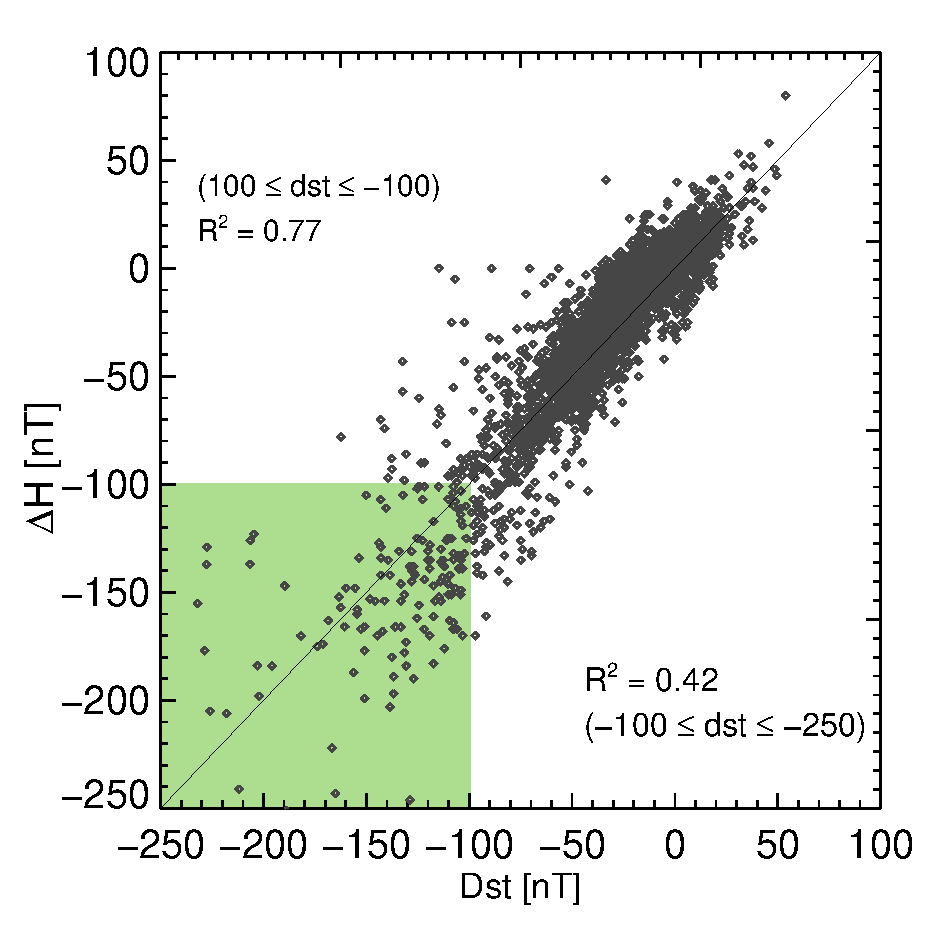
\includegraphics[width=0.7\textwidth]{Images/dispersion_general_dst.eps}
      \caption{Gráfica de dispersión de $\Delta$H (eje vertical) con respecto a Dst (eje horizontal) para todos los eventos TG. La región verde representa un umbral de -100 nT en que fue calculado $R^2$.}
       \label{fig:disp}
\end{figure}


\section{Identificación de firmas magnéticas}

Los valores locales del CMT resultan del efecto combinado de diferentes fuentes que contribuyen al campo total \parencite{iaga_guide, 1969intro_to_iono_p, l_handbook_geof_sw_Geom_field, baseline_Gjerloev, vanKampt}. Estas fuentes contribuyen a la componente H del CMT local, lo cual puede expresarse como:

\begin{equation}
    \label{eq:1}
        H = H_{SQ} + H_0 + D_{M} + D_{I},
\end{equation}

donde $H_{SQ}$ representa la variación diurna derivada de los días quietos locales \cite{vanKampt}, mientras que $H_0$ representa las variaciones día a día \parencite{baseline_Gjerloev}. Los últimos términos representan las perturbaciones asociadas con la TG y representan la contribución de las corrientes magnetosféricas e ionosféricas respectivamente \parencite{ddyn2005, angeoddyn}. La contribución de $D_M$ para latitudes geomagnéticas medias y bajas puede aproximarse de la siguiente forma $Dst \cdot \cos(\lambda)$, donde $\lambda$ es la latitud geomagnética de donde fueron tomados los datos \parencite{amorymazaudier_2017}. 
\vspace{1 em}

Considerando lo mencionado en secciones anteriores, la contribución de interés es la asociada con mecanismos ionosféricos o $D_I$, por lo que el siguiente paso es simplemente aislarlo del resto de contribuciones magnéticas. Para ello, a partir de la expresión \ref{eq:1}:

\begin{equation}
\label{eq:diono}
   D_{I} \approx H -(H_{SQ} +  H_0 + Dst \cdot cos(\lambda)).
\end{equation}

Además, de acuerdo con \cite{ddyn2005, angeoddyn}, en latitudes medias y bajas, $D_I$ es la suma de las firmas magnéticas de CPP2 y CDP:
\begin{equation}
\label{eq:diono_explicit}
   D_{I} = H_{Ddyn} + H_{DP2} + H_{otras},
\end{equation}

donde $H_{otras}$ se refiere a cualquier otra perturbación de origen ionosférico, diferente de \emph{Ddyn} y \emph{DP2}.
\vspace{1 em}

Para aislar de forma efectiva las firmas magnéticas atribuidas a $H_{Ddyn}$ y a $H_{DP2}$ en las ecuaciones \ref{eq:diono} y \ref{eq:diono_explicit}, se empleó de forma inicial un filtro de frecuencias para analizar $D_I$ \parencite{amory2020_filtros}. Estos filtros fueron diseñados de acuerdo con los rangos de frecuencias (periodos) en que las corrientes \emph{Ddyn} y \emph{DP2} ocasionan fluctuaciones en las observaciones locales del CMT \parencite{nishida_68_fluctuations, blanc_ddyn, ddyn_diag2}. En el caso de \emph{Ddyn}, se trata de filtros pasa-bandas entorno a las 24h, mientras que para \emph{DP2} se usa un filtro pasa-altas, para periodos de fluctuación menores de 4h. 

\subsection{Resultados, resolución: 1 h}
\label{resultados}
A continuación, se muestra el proceso de análisis, poniendo como ejemplo el evento 13, ocurrido el 16 de marzo del 2015. Se trata del evento conocido como la tormenta de San Patricio. En el panel(a) de la Figura \ref{fig:iono_resp}
\vspace{1 em}

\begin{figure*}
\centering
    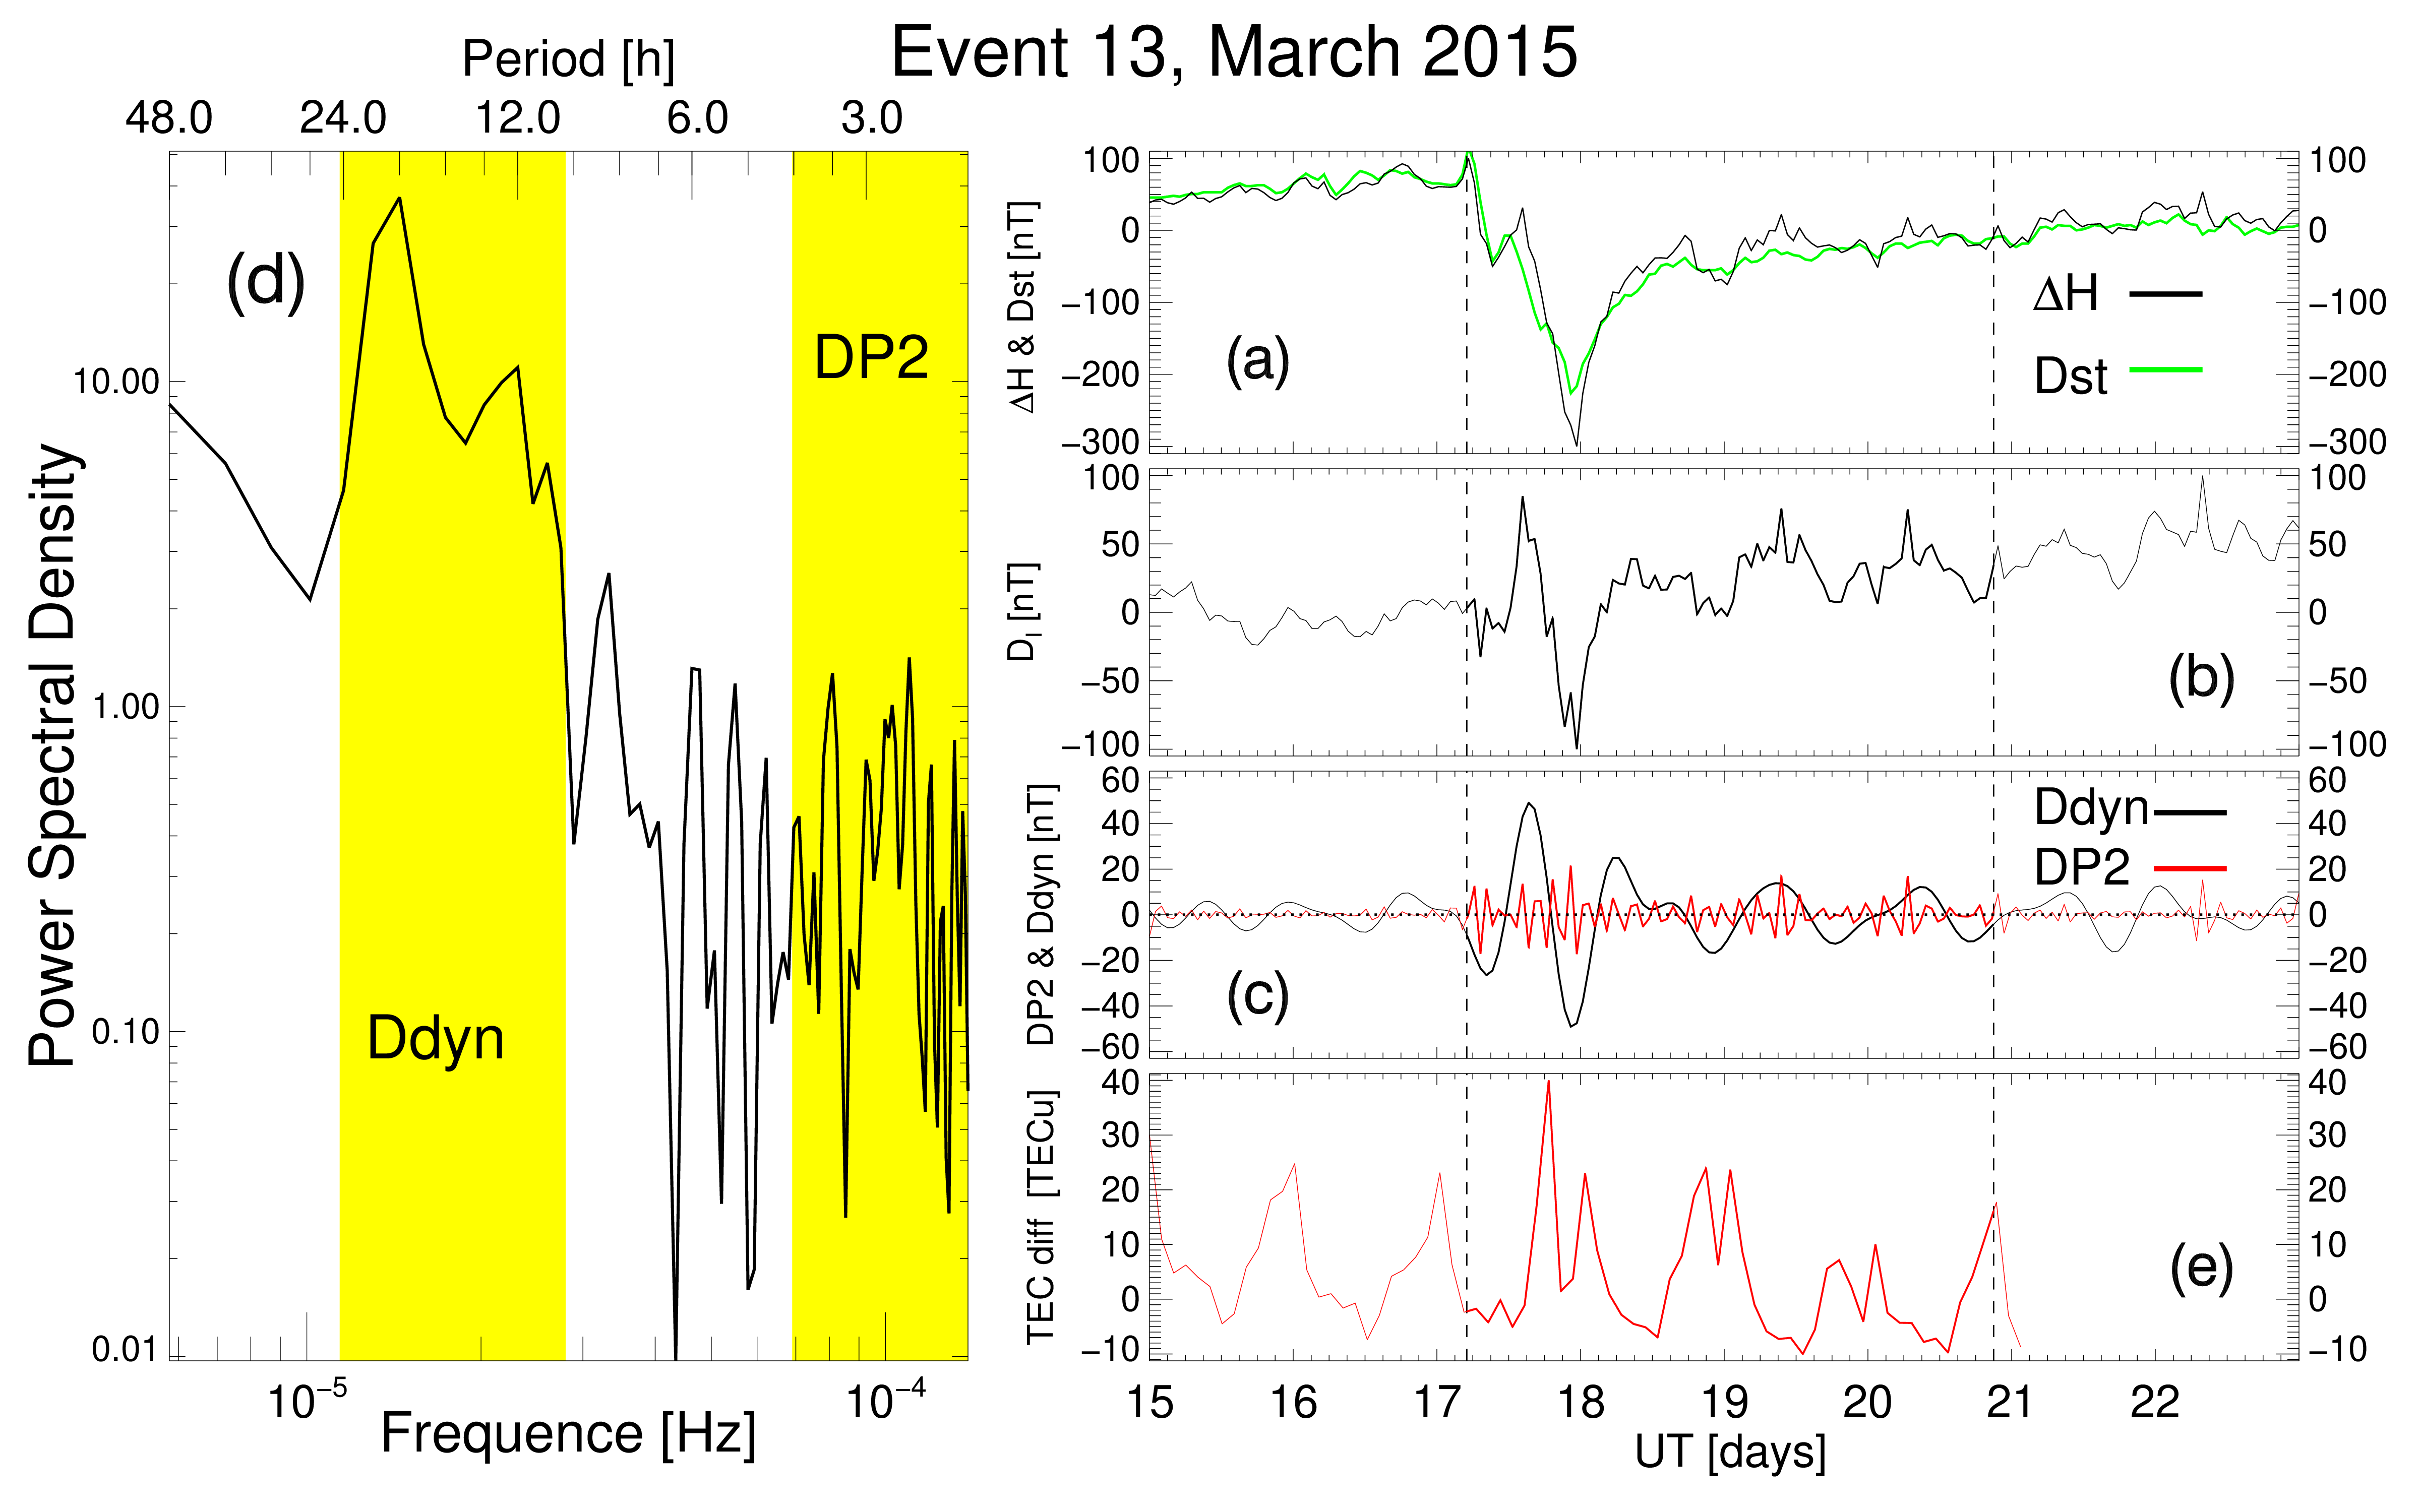
\includegraphics[width=0.85\textwidth]{Images/iono_PI_2015-03-15.png}
    \caption{Análisis del caso de estudio 13. Panel (a): $Dst$ (negro) y $\Delta H$ (verde). Panel (b): valor calculado de $D_I$. Panel (c): Perfiles reconstruidos de los efectos magnéticos de Ddyn (linea negra) y DP2 (linea roja). Panel (d): Espectro de Densidad de Potencia de $D_I$ o PSD. Panel (e): Medida de la diferencia de Contenido Total de Electrones (TEC) encima del centro de México. Las líneas verticales discontinuas indican el periodo de mayor impacto de la TG en el CTM. Las regiones amarillas en el panel (d) resaltan los anchos de bando asociados con  $Ddyn$ (25h - 10 h) y $DP2$ (menos de 4.5 h).}
    \label{fig:iono_resp}
\end{figure*}

En el panel (b) de la Figura \ref{fig:iono_resp}, se aprecia el resultado del perfil $D_I$ (Ecuación (\ref{eq:diono})), calculado a partir de las observaciones de TEO y los datos reportados del índice $Dst$. Subsecuentemente, se construyó un espectro de potencia \emph{PSD}. Para su construcción, tal y como se indica en la Sección \ref{psd_section} se utilizó una función ventana (Ventana de Hanning) para atenuar la dispersión de energía en los picos de potencia de interés. Las regiones de color amarillo resaltan los rangos de periodos (frecuencias), que son consistentes con los rangos de fluctuación del CMT regional debido a la presencia de \emph{Ddyn} y \emph{DP2}. En el panel se identifica el rango de frecuencias de \emph{Ddyn} al ajustar el periodo principal e identificar los picos de potencia. Es importante tomar en cuenta que, debido a la diferencia de los casos de estudio, pueden haber diferencias significativas en los rangos de \emph{Ddyn} para cada TG. Es por ello que los anchos de banda ajustados para cada TG pueden variar. 
\vspace{1 em}

En la Figura \ref{fig:iono_resp}(c) se presentan los perfiles de las perturbaciones ocasionadas por \emph{DP2} (linea roja) y \emph{Ddyn} (linea negra). Estos perfiles fueron construidos a partir de los rangos de frecuencias identificados a través de los procesos de filtros comentados en el párrafo anterior. Se puede observar que los incrementos de los efectos inducidos por \emph{Ddyn} y \emph{DP2} ocurren de forma simultanea con un incremento del $TEC_{dif}$ sobre el centro de México mostrado en el panel (e) de la Figura \ref{fig:iono_resp}, mencionado en la sección \ref{diono}. 
\vspace{1 em}

%El procedimiento previamente mostrado fue aplicado a los 20 casos de estudio usando datos de TEO. En las Figuras \ref{fig:iono_resp2} y \ref{fig:iono_resp3} del apéndice, se muestran los perfiles calculados de $D_I$, así como los perfiles de \emph{Ddyn} y \emph{DP2} de cada evento mostrado en la Tabla \ref{table1:GS_descp}. Al observar cada evento, se resaltan sus particularidades individuales, las cuales son evidentes en los perfiles de $D_I$ y sus perturbaciones magnéticas asociadas con \emph{Ddyn} y \emph{DP2}.
%\vspace{1 em}

A partir de las observaciones de los 20 eventos de la Tabla \ref{table1:GS_descp}, se encontró que generalmente, la amplitud de las oscilaciones magnéticas inducidas por \emph{Ddyn} son más intensas que aquellas inducidas por \emph{DP2}. Esto sugiere que, en la mayoría de los casos, los efectos de inducción magnética de \emph{Ddyn} son dominantes en el CMT local. Aunque también hay eventos para los cuales ambos efectos tienen intensidades similares. Se piensa en dos posibilidades para explicar estos resultados: El primero, es el mecanismo que desencadena la TG en sí, \emph{i.t.} y su reconexión magnética con el CMT. Esto puede afectar la evolución de la respuesta ionosférica, modificando directamente la evolución de las corrientes \emph{Ddyn} y \emph{DP2}. En segundo lugar, se debe considerar que los datos usados en un inicio tienen una resolución de 1h. En este caso, el muestreo de datos representa una limitación importante ya que las fluctuaciones magnéticas ocasionadas por \emph{DP2}, tal y como se menciona en \cite{nishida_68_fluctuations}, pueden tener periodos de menos de una hora hasta incluso unas poca decenas de minutos. En este escenario, es posible que se pierdan parte de las fluctuaciones más significativas inducidas por \emph{DP2}. Esto se puede resolver al usar datos del índice $SYM-H$ en vez de $Dst$, así como datos locales de 1 minuto de resolución, caso del cual se estará hablando en la sección \ref{PSD2}. 
\vspace{1 em}

\section{Validación de resultados} \label{validacion}

En la sección \ref{respuesta_dif}, identificamos diferencias substanciales entre la respuesta planetaria y la regional. En la sección \ref{resultados}, se determinaron los mecanismos geomagnéticos que tentativamente den origen a esas variaciones regionales, además de señalar su consistencia con la respuesta ionosférica medida mediante $TEC_{dif}$. Para validar estos resultados, se realizó una aproximación de múltiples pasos.  
\vspace{1 em}

Inicialmente, se aproximó el índice regional $\Delta H_{TEO}$ al definirlo como se muestra a continuación:

\begin{equation}
    \label{eq:deltaH}
    \Delta H_{TEO} = H_{TEO} - (H_{SQ} + H_0),
\end{equation}

Usando las ecuaciones (\ref{eq:diono}), (\ref{eq:diono_explicit}), y (\ref{eq:deltaH}), se deriva:

\begin{equation}
    \label{eq:deltaHandDst}
    \Delta H_{TEO} \approx Dst \cos(\lambda) + DP2 + Ddyn.
\end{equation}

Para simplificar, se denotó a $ Dst_\lambda$ como el efecto combinado de $ Dst\cos(\lambda)$, $DP2$, y $Ddyn$. Esto condujo al primer paso de validación, confirmando si el $ Dst_\lambda$ se aproximaba a $\Delta H$. Adicionalmente, se empleó a $ Dst_\lambda$ y los valores de $K_P$ para aproximar el valor local de $K$. 
\vspace{1 em}

La figura \ref{fig:iono_valid} muestra el proceso de validación aplicado para el evento 13. En el panel superior se observan sobrepuestos los perfiles de $\Delta H_{TEO}$ (negro), $Dst$ (verde), y $Dst_\lambda$ (rojo). Es evidente que, $Dst_\lambda$ consistentemente tiene un comportamiento más parecido a $\Delta H_{TEO}$ que $Dst$ , siendo esto válido para el periodo señalado por las lineas verticales discontinuas que enmarcan la fase principal y parte de la fase de recuperación de la TG. En el panel inferior se muestra que los valores $K$ planetarios (verde) y regionales (negro) difieren. Sin embargo, cuando $Dst_\lambda$ es combinado con $K_P$ usando las barras de incertidumbre, el perfil de $K$ local se ubica dentro de este rango.
\vspace{1 em}

\begin{figure}
\centering
    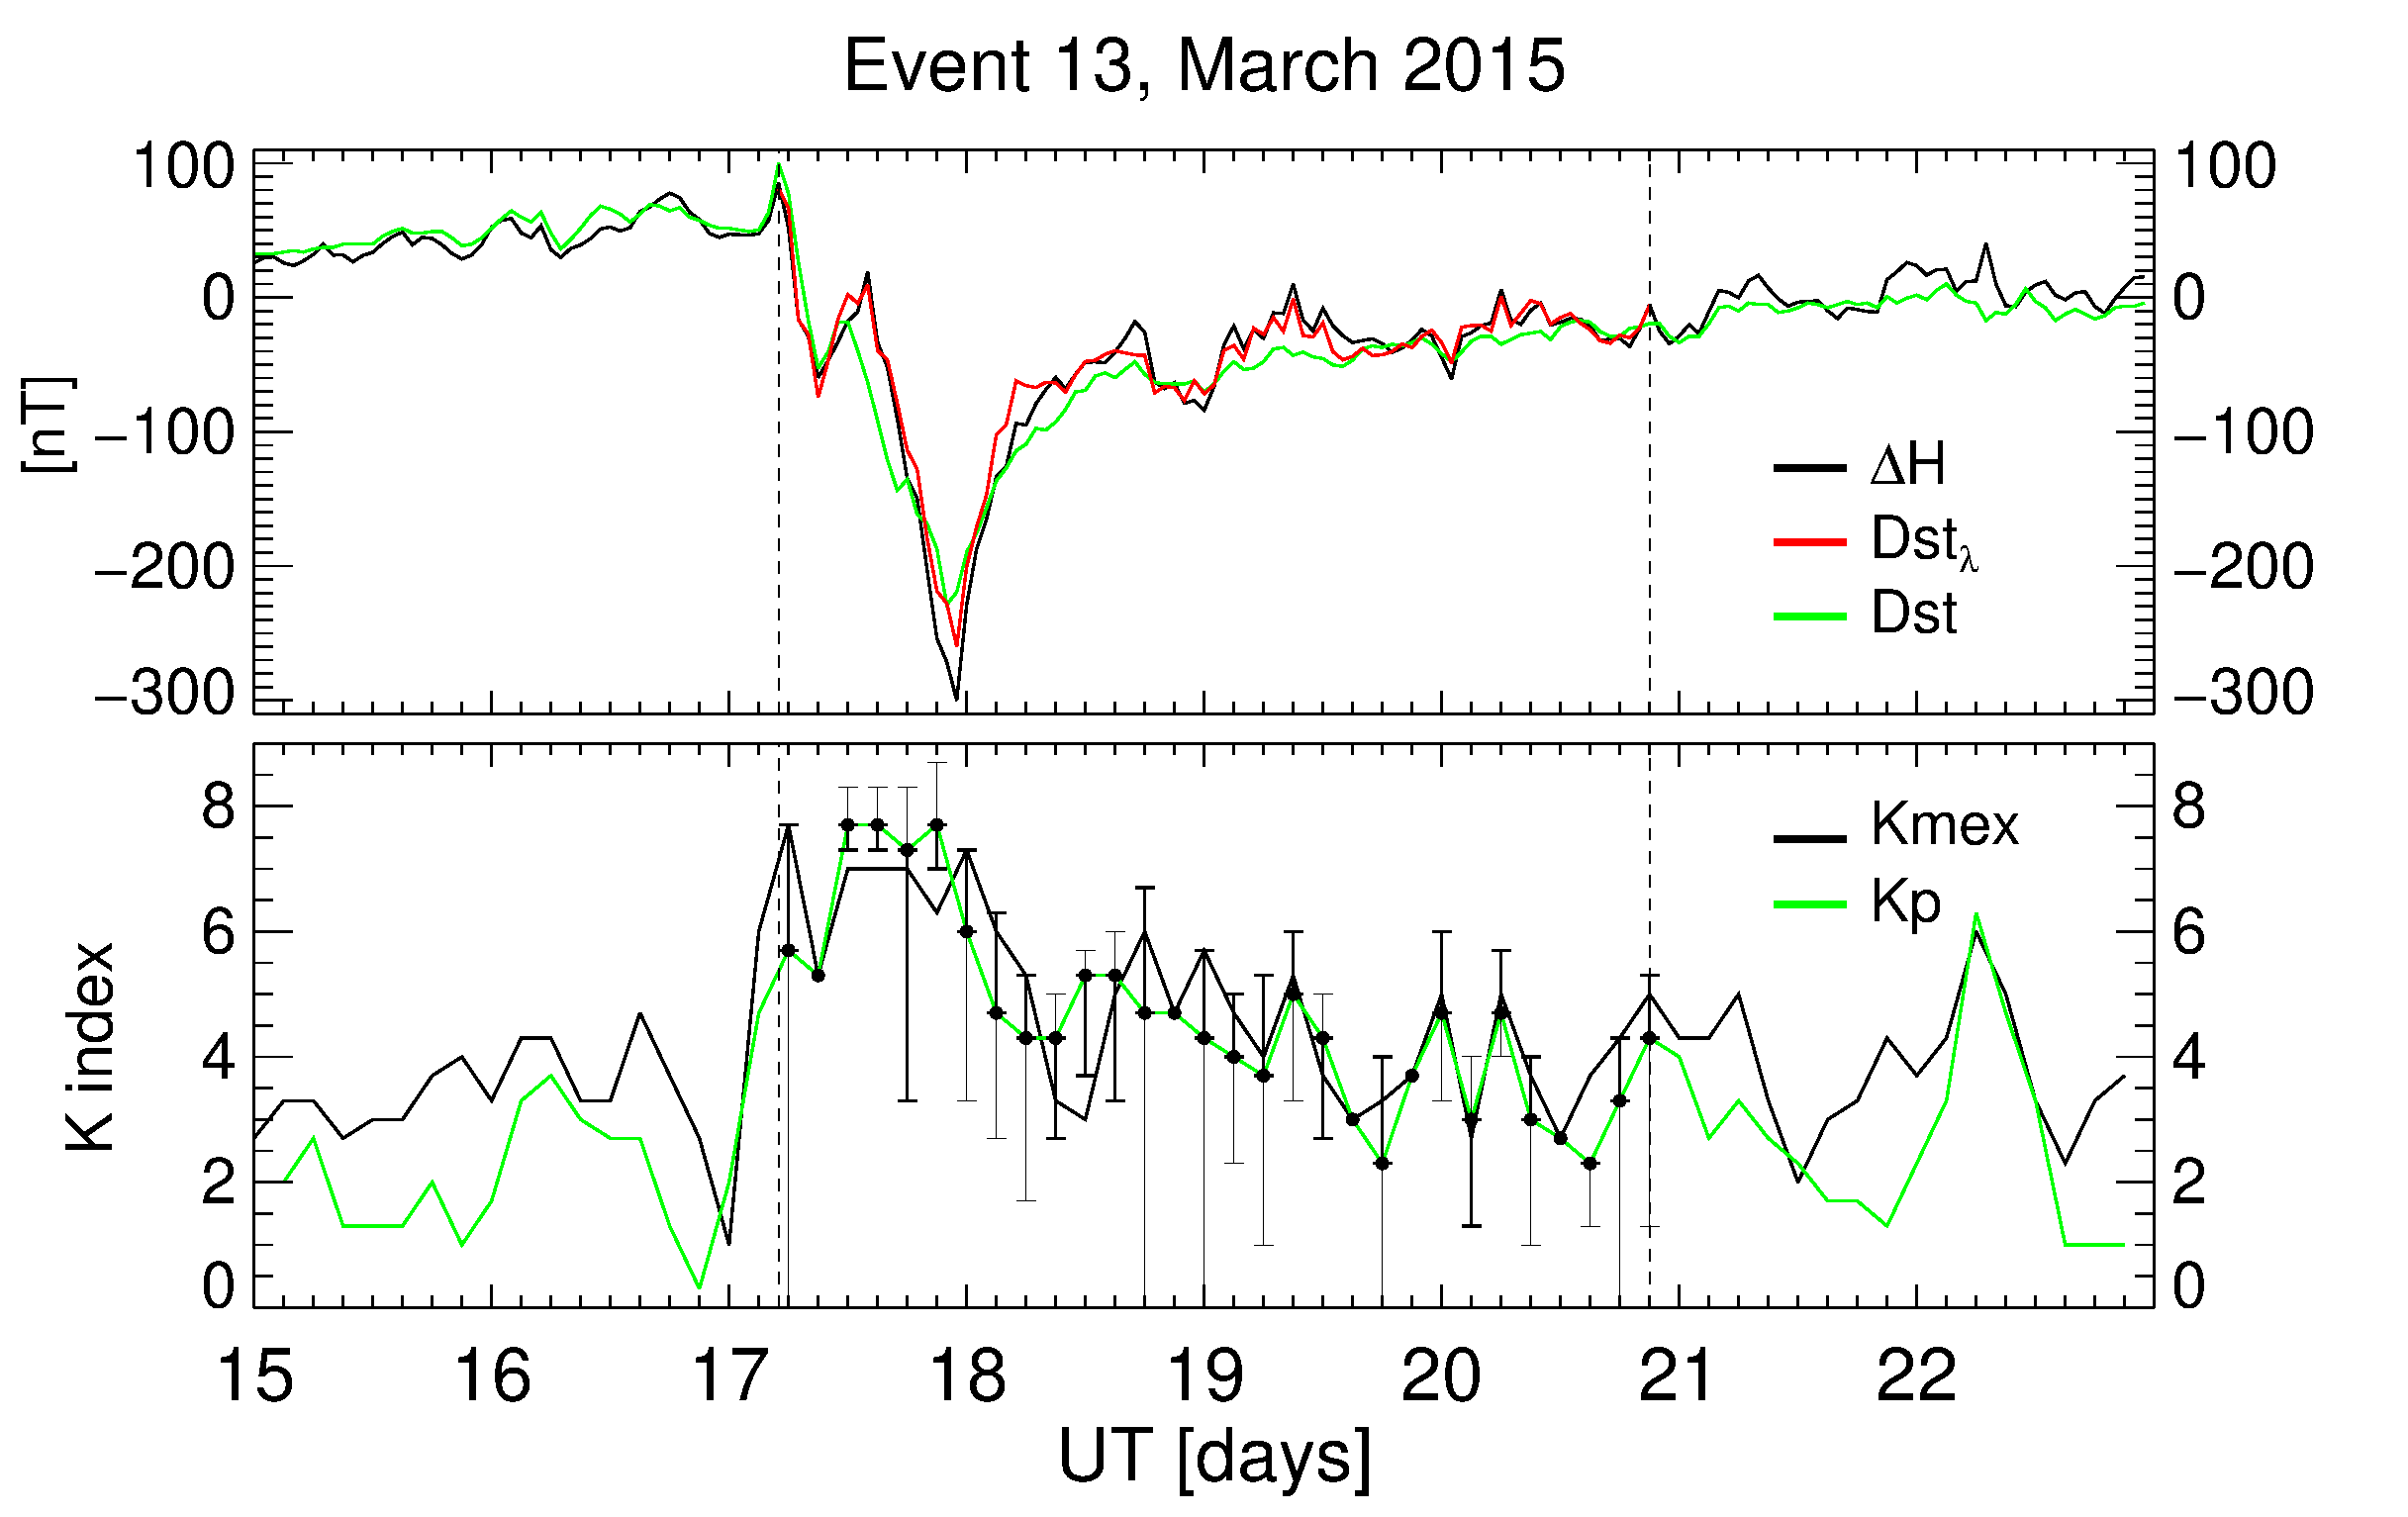
\includegraphics[width=0.7\textwidth]{Images/diono_valid_V4_2015-03-15.eps}
    \caption{Aproximación de los índices geomagnéticos  $\Delta H_{TEO}$ (arriba) y el $K_{TEO}$ (abajo). Las lineas verdes representan los índices planetarios mientras que las líneas negras representan los índices locales. El índice aproximado $\Delta H_{TEO}$ es representado mediante la linea roja, mientras que las barras de error representan un rango de aproximación para el índice $K_{TEO}$.}
    \label{fig:iono_valid}
\end{figure}

Para  validar de forma comprensiva, este proceso es aplicado a todos los casos de estudio. Consistentemente, $ Dst_\lambda$ se aproxima a $\Delta H_{TEO}$; mientras que $K_p$ combinado con los efectos de $Dst_\lambda$ envuelve los valores regionales de $K_{TEO}$.
\vspace{1 em}

Adicionalmente, se condujo un método cuantitativo de comparación. Se calculó el error promedio absoluto de la diferencia entre $\Delta H_{TEO}$-$Dst$ y $\Delta H$-$Dst_\lambda$ [nT]. Como se ilustra en la Figura \ref{fig:valid}

\begin{figure}
\centering
    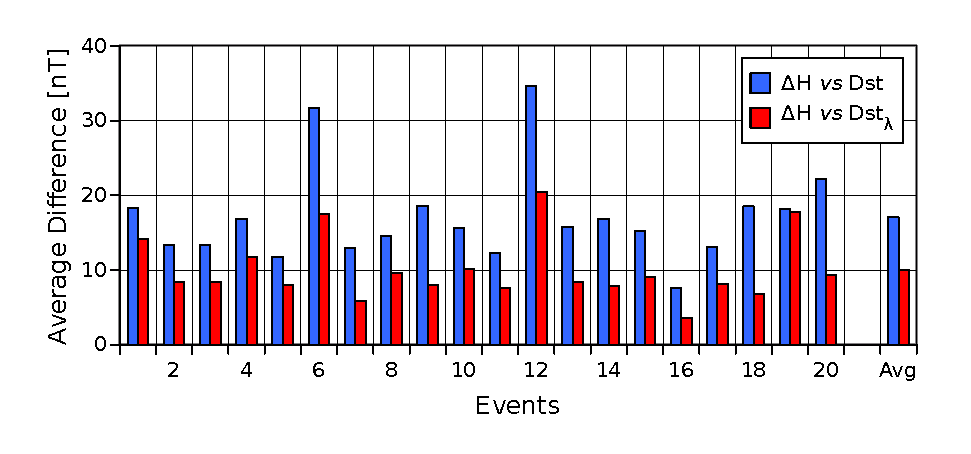
\includegraphics[width=0.7\textwidth]{Images/prom_dist.eps}
    \caption{Error promedio medido en nT entre $\Delta$H vs Dst (barras azules) y $\Delta$H vs $Dst_\lambda$ (barras rojas).}
    \label{fig:valid}
\end{figure}

En la figura \ref{fig:valid} se puede observar que el promedio absoluto del error entre $\Delta H_{TEO}$-$Dst_\lambda$ es menor que $\Delta H_{TEO}$-$Dst$. Esto indica un comportamiento más parecido por parte de $Dst_\lambda$ con respecto de la respuesta geomagnética regional observada. 
\vspace{1 em}

El paso final involucra resaltar la gráfica de dispersión de la Figura \ref{fig:disp}, empleando a $Dst_\lambda$ en vez de $Dst$. El resultado se muestra en la Figura \ref{fig:valid_disp2} , los datos puntuales (diamantes) más cercanos a la identidad (linea negra), en contraste con la Figura \ref{fig:disp}. Más aún, $R^2$ tiene un incremento de 0.77 a 0.86 para el rango de $Dst \ge -100\, {\rm nT}$, mientras que para el rango de $Dst < -100\, {\rm nT}$, $R^2$ tiene un aumento significativo de 0.75, con respecto a su valor original ($R^2=0.42$).
\vspace{1 em}

\begin{figure}
    \centering
     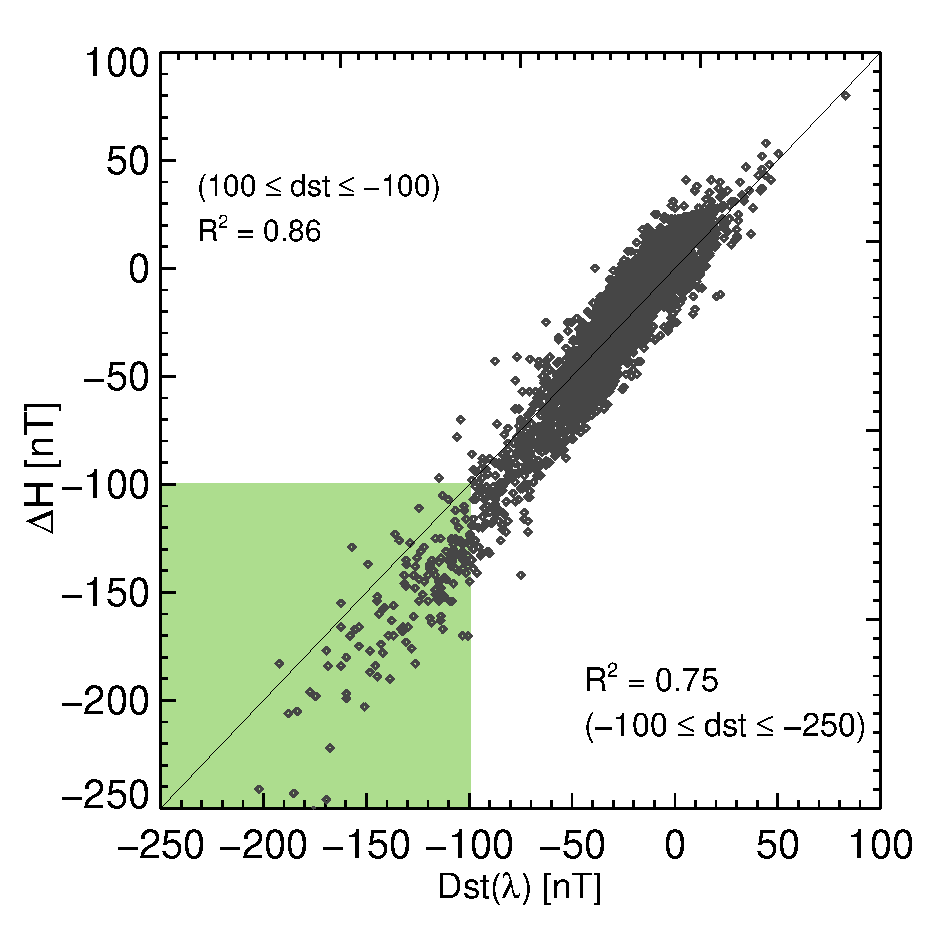
\includegraphics[width=0.7\textwidth]{Images/dispersion_general_dst_ld.eps}
      \caption{Gráfica de dispersión $\Delta H_{TEO}$ (eje vertical) con respecto a $Dst_\lambda$ (eje horizontal) para todos los eventos TG. La región verde representa un umbral de -100 nT en que fue calculado el segundo $R^2$.}
       \label{fig:valid_disp2}
\end{figure}

Con el proceso de validación, se demostró que las perturbaciones magnéticas potencialmente inducidas por las corrientes ionosféricas $DP2$ y $Ddyn$, cuando se combinan con la respuesta planetaria (índice $Dst$) permiten una aproximación cuantitativa aceptable de la respuesta geomagnética regional. Más aún, las diferencias entre los datos regionales y planetarios se reducen de forma sustancial al integrar los efectos magnéticos de $DP2$ y $Ddyn$ en la respuesta planetaria.
\vspace{1 em}

\section{Análisis de espectral II}
\label{PSD2}

\subsection{Potencia espectral, resolución: 1 min}

Con el uso de datos con resolución de 1 minuto, el primer paso fue el de realizar un estudio más detallado de los PSD. En la Figura \ref{fig:powerlaw} se muestra el PSD aplicado para el evento 21, ocurrido en 2023 y para el cual se utilizan datos de COE. En el panel de arriba se muestra la serie de tiempo, una vez removidos los efectos $H_{SQ}$, mientras que en el panel inferior se observa la misma serie de tiempo sin remover $H_{SQ}$.
\vspace{1 em}

Una de las primeras observaciones es que, independientemente del panel (o del evento en cuestión), en ambos casos se muestra lo que parece ser dos leyes de potencia, asociadas a los rangos de frecuencia en que se presentan las fluctuaciones inducidas por \emph{Ddyn} y \emph{DP2}. En la Figura las leyes de potencia se representan mediante las lineas rojas continuas que se denominaron como $a1$ y $a2$. Las leyes de potencia fueron calculadas a partir de mínimos cuadrados, de acuerdo al criterio utilizado por \cite{LS_red_noise}. El par de lineas segmentadas señala el error de la ley de potencia. Cabe señalar que, $a1$ y $a2$ se ven afectadas por la presencia del efecto $H_{SQ}$, pues en la Figura \ref{fig:powerlaw}, la integración del efecto $H_{SQ}$ provoca un desajuste con respecto de la \emph{PSD}. Otra consideración a tomar en cuenta es que las leyes de potencia calculadas también se ven altamente afectadas por los picos negativos, en determinados eventos.
\vspace{1 em}

 
Se puede observar un fenómeno interesante entre $a1$ y $a2$ (en la banda de periodo de entre las 6h y las 3 h) un fenómeno recurrente en los eventos. Es la presencia de lo que parece ser, un efecto escalón, donde entre cada ley de potencia pareciera presentarse otra potencia. De igual forma, para fluctuaciones de periodo menor a 20 minutos, se observa en general otra ley de potencia más, la cual pareciera estar más cercana al ruido blanco. En general, diferentes leyes de potencia en un PSD son un indicativo de fluctuaciones persistentes, por lo que se espera conseguir información de interés asociado a las leyes de potencia presentes en cada PSD.
\vspace{1 em}

\begin{figure}
    \centering
     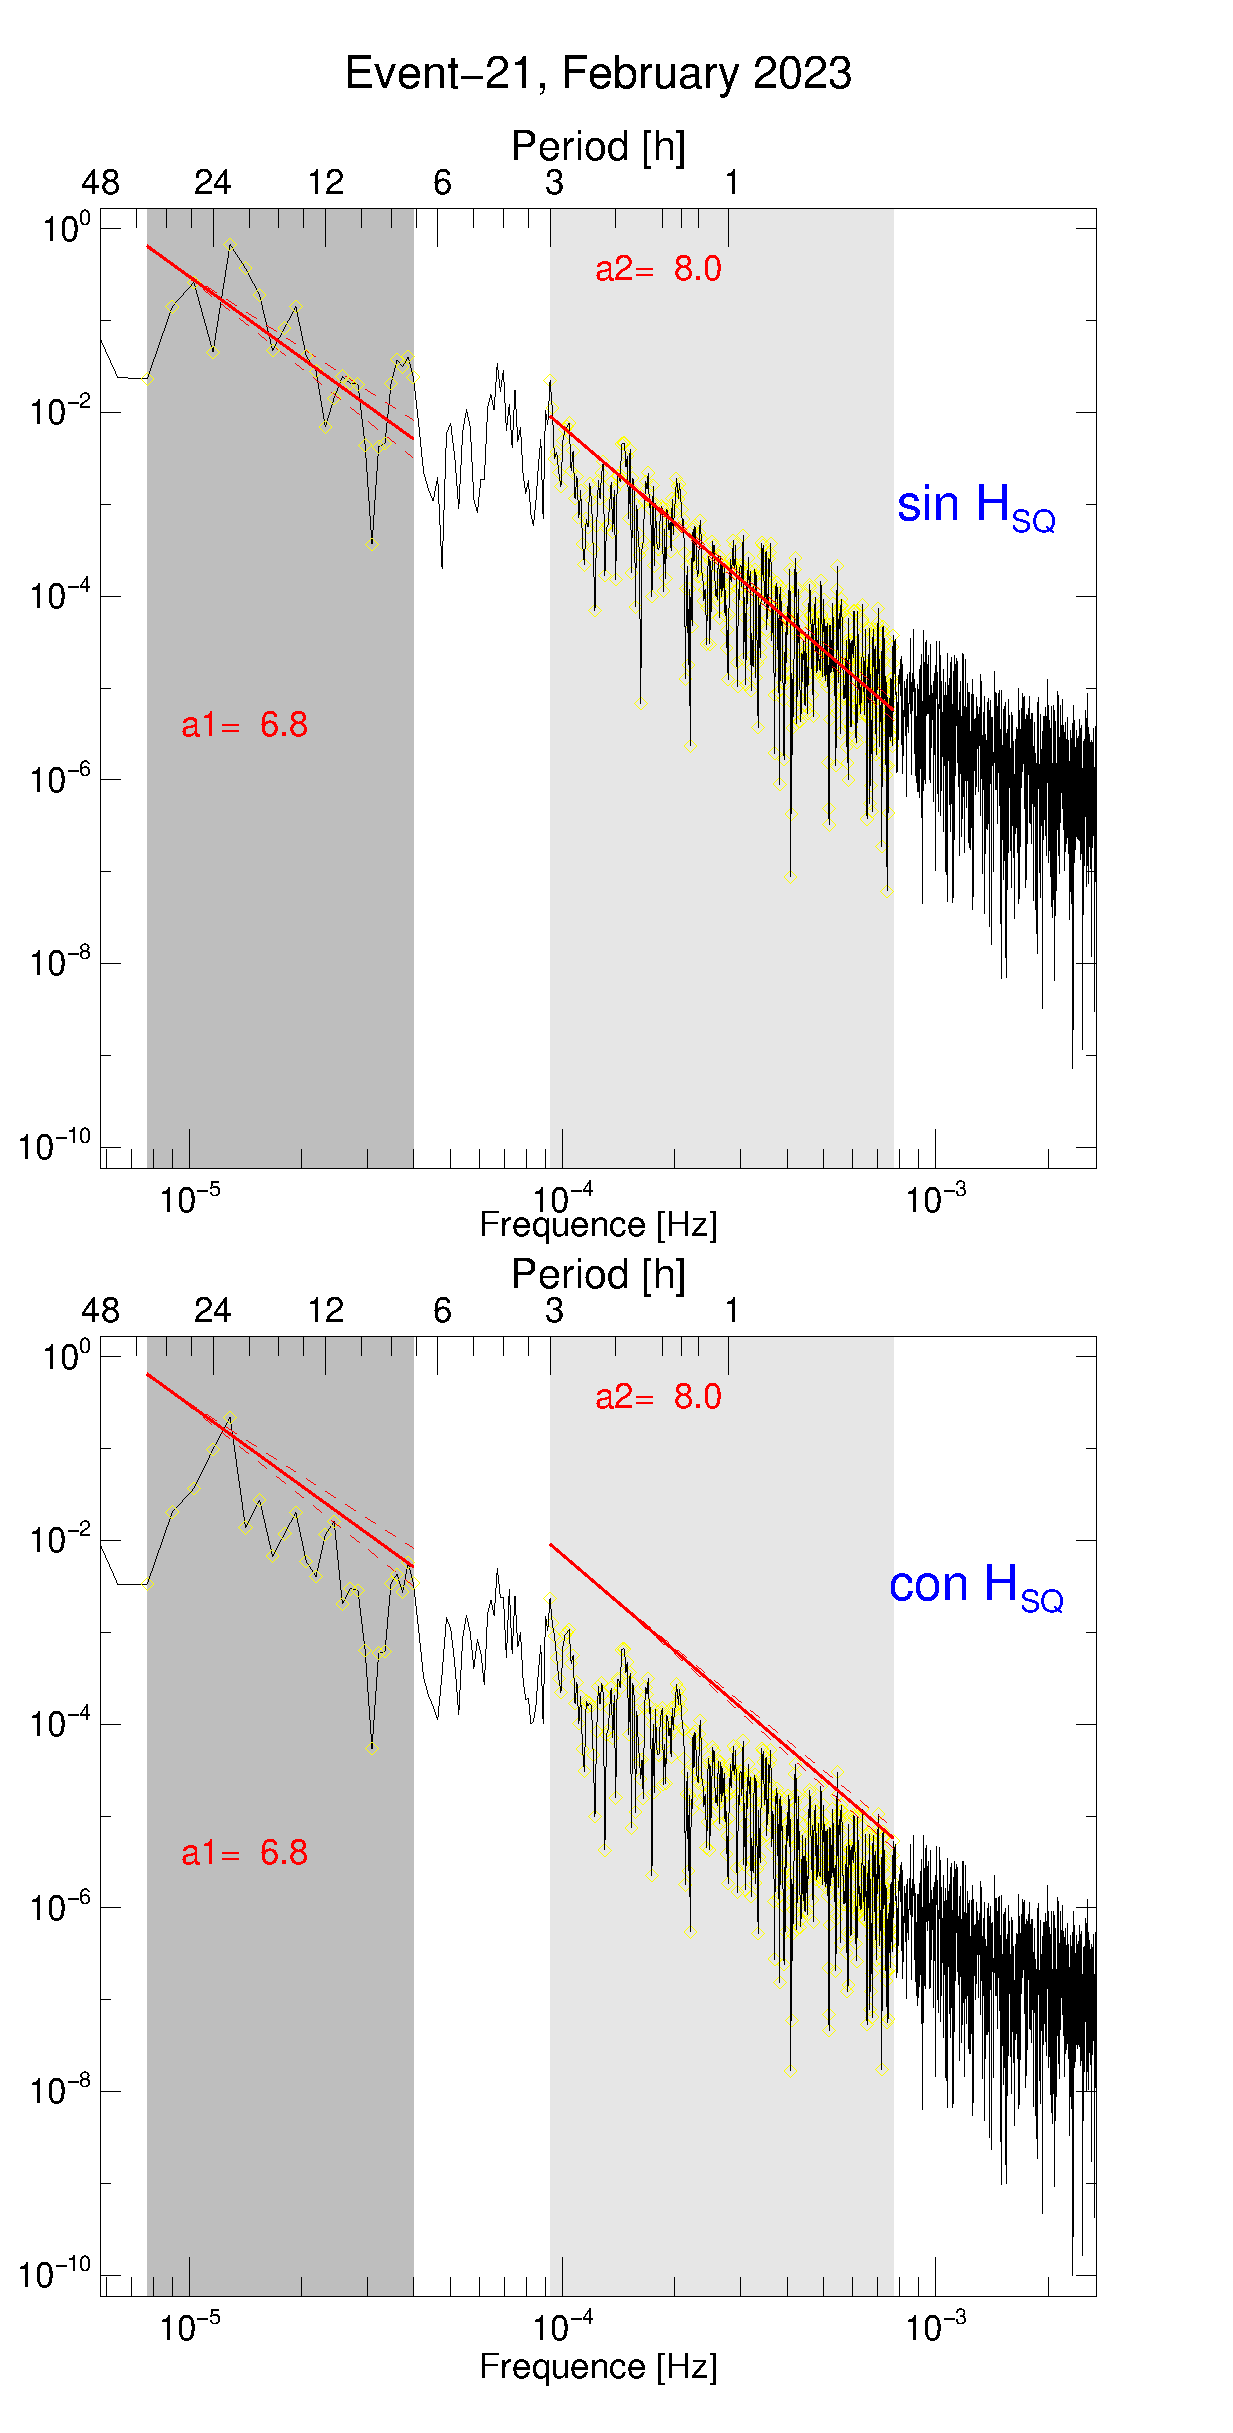
\includegraphics[width=0.65\textwidth]{Images/cap3/powerlaw/diono_PWS_powerL_2023-02-25.eps}
      \caption{Espectro de potencia (linea negra), considerando para la serie de tiempo removiendo el efecto $H_{SQ}$ (arriba) y sin removerlo (abajo). Las líneas rojas representan las leyes de potencia asociadas con \emph{Ddyn} (a1) y \emph{DP2} (a2). Las regiones gris oscuro y gris claro resaltan los anchos de banda que abarcan estas leyes de potencia.}
       \label{fig:powerlaw}
\end{figure}


\subsection{Análisis de ondículas}

A partir del trabajo realizado por \cite{2021amory}, donde se concluyó que un análisis de ondículas sería más adecuado para este tipo de fenómenos, se optó por hacer lo propio para los 23 eventos en México. En este caso se utilizó la ondícula de Morlet como ondícula madre. En la Figura \ref{fig:wave} se muestra el resultado de aplicar un análisis de ondícula, mientras que en la Figura \ref{fig:wavepower} se muestra la potencia espectral de la ondícula. La malla que se observa en ambas figuras es la región afectada por el efecto borde, o Cono de Influencia. 
\vspace{1 em}

Se observa en la Figura \ref{fig:wave} un efecto consistente en periodos de entre 28h y 12h con la presencia de una TG entre el 26 de febrero y el 4 de marzo del 2023. Los tonos cálidos y fríos son consistentes con los periodos de día y noche, los cuales son importantes en el fenómeno de \emph{Ddyn}. Además, se puede observar los días en que éste fenómeno tuvo una mayor amplitud. Por otro lado, se observan fluctuaciones en el rango de las 4h hasta menos de 1h, los cuales se limitan a aquellos periodos donde se presenta una reconexión magnética, lo cual es consistente con el fenómeno \emph{DP2}. 
\vspace{1 em}

En algunos casos (eventos 4, 5, 6, 13, 15, 19) se observó un efecto persistente de periodo entorno a las 48h - 72h. Esto también fue observado en los PSD de los respectivos eventos. Una primera hipótesis planteada sería un efecto no suficientemente bien atenuado de la línea base día a día. Sin embargo, este rango entra dentro del Cono de Influencia, por lo que no debería ser tomado en cuenta.  
\vspace{1 em}

En esos mismos eventos, también se observa una potencia en la banda de frecuencias asociada con \emph{Ddyn}. Esto en principio podría indicar que durante los eventos 4, 5, 6, 13, 15, 19; el efecto magnético inducido por \emph{Ddyn} no fue muy significativo dentro de las variaciones magnéticas locales. 
\vspace{1 em}



\begin{figure}
    \centering
     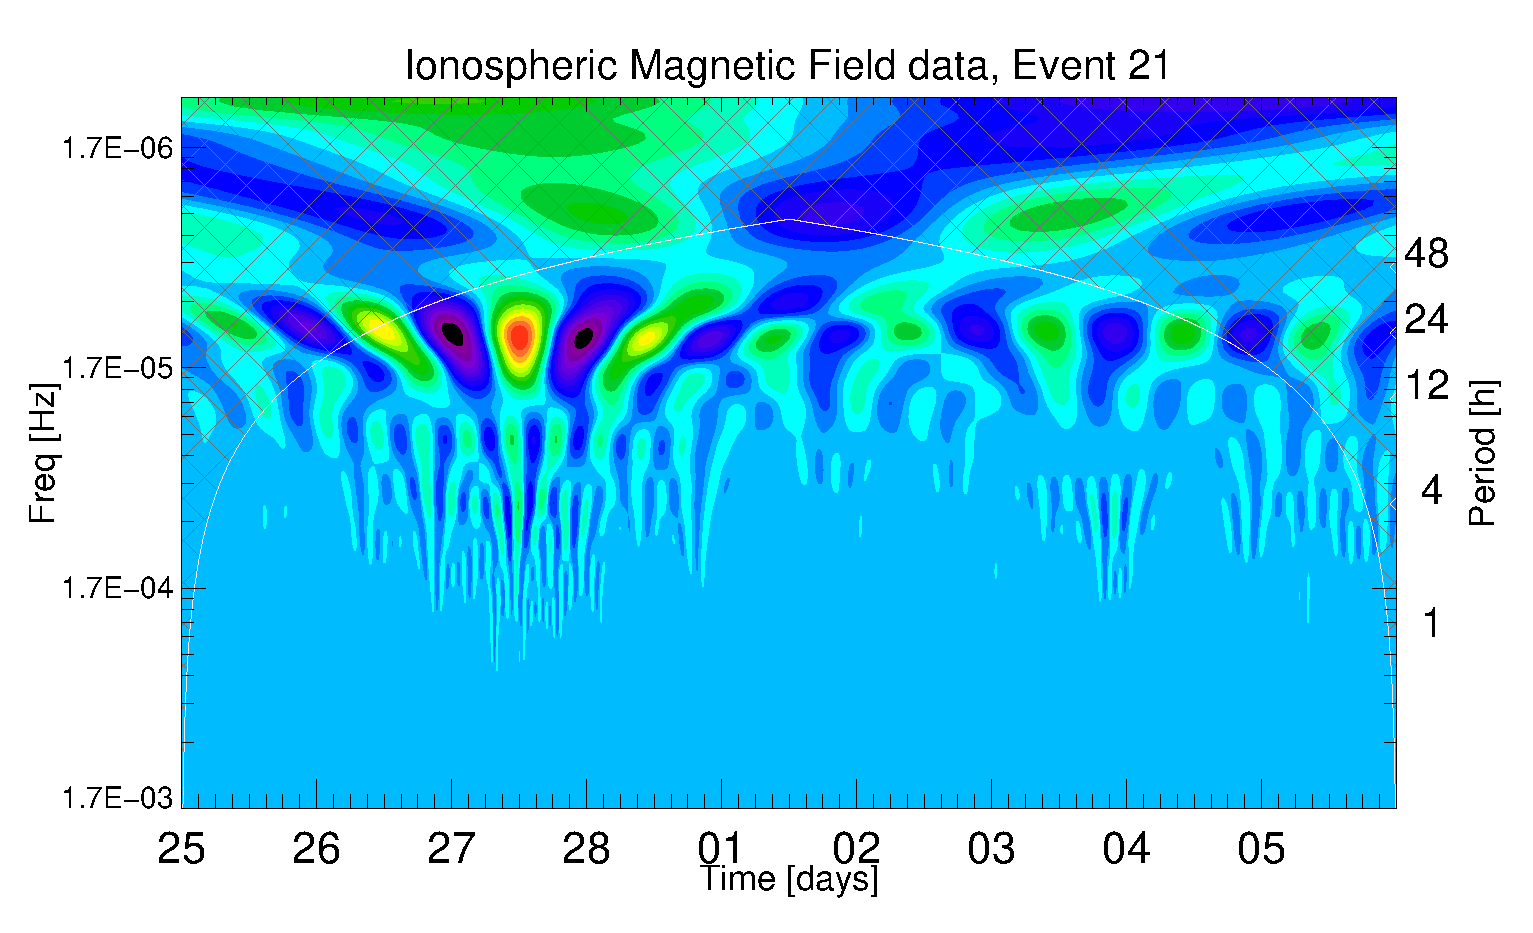
\includegraphics[width=0.7\textwidth]{Images/cap2/wave/wave_2023-02-25.uncut.eps}
      \caption{Análisis de ondícula aplicado a la TG 21. El mayado en la parte superior representa el Cono de influencia ocasionado por el efecto de borde.}
       \label{fig:wave}
\end{figure}

Por otro lado, también se calculó la potencia espectral de la ondícula, lo cual se ve plasmado en la Figura \ref{fig:wavepower}. En la Figura se observa claramente los días en que \emph{Ddyn} tuvo un mayor impacto en el CMT local. Por otro lado, no se observan fluctuaciones relevantes en el rango de fluctuación de \emph{DP2}.
\vspace{1 em}

Por último, algo que es necesario observar en este evento y que también fue observado en los eventos 1, 3, 11, 18 y 23 es la presencia de aparentes armónicos, potencialmente asociados con \emph{Ddyn}. Este y otros aspectos serán investigados posteriormente.


\begin{figure}
    \centering
     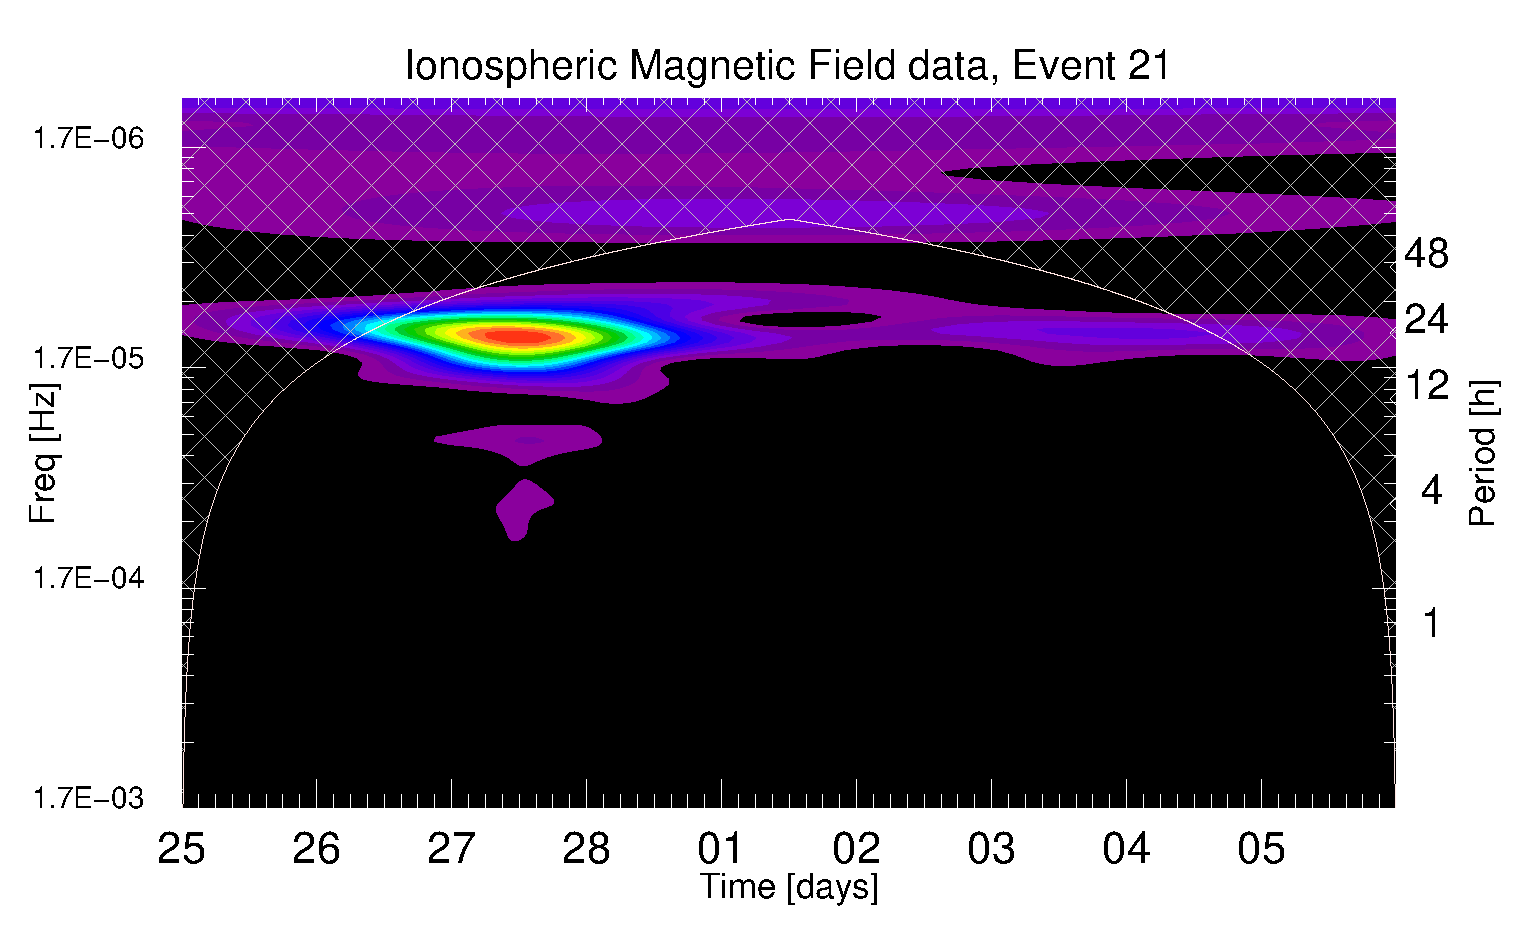
\includegraphics[width=0.7\textwidth]{Images/cap2/power/power_2023-02-25.uncut.eps}
      \caption{Análisis de potencia y significancia de ondícula, aplicado a la TG 21. El mayado en la parte superior representa el Cono de influencia ocasionado por el efecto de borde.}
       \label{fig:wavepower}
\end{figure}

\section{Observaciones finales}
En este primer trabajo, se estudiaron las manifestaciones regionales de clima espacial. El enfoque fueron las diferencias en la respuesta geomagnética regional con respecto a la planetaria durante periodos de Tormentas Geomagnéticas (TG) intensas sobre el centro de México. También se investigaron los mecanismos físicos responsables de tales variaciones geomagnéticas. Se utilizaron los registros geomagnéticos del observatorio geomagnético de Teoloyucan (TEO), localizado al norte de la Ciudad de México. También se están empleando datos de la estación geomagnética de Coeneo (COE), localizada en Michoacán. También se utilizaron los datos de los índices planetarios $Dst$ y $K_P$, los índices regionales $\Delta H_{TEO}$ y $\Delta H_{COE}$, así como el Contenido Total de Electrones, proporcionado por el Laboratorio Nacional de Clima Espacial (LANCE).
\vspace{1 em}

Se seleccionaron en principio 20 casos de estudio (véase la Tabla \ref{table1:GS_descp}) para el caso de los datos de TEO, más 3 casos (Tabla \ref{table2:GS_descp}) con datos de COE. Para todos los casos de estudio, se identificó la evidencia de una respuesta geomagnética regional relevante a través de la gráfica de dispersión (Véase la Figura \ref{fig:disp}). En este caso, se encontró que en el rango de $Dst < -100 {\rm nT}$, hay una tendencia para el índice geomagnético regional a desviarse del planetario. Se asume este comportamiento como evidencia de una respuesta geomagnética regional.
\vspace{1 em}

Subsecuentemente, se validaron las contribuciones geomagnéticas debidas a las corrientes $Ddyn$ y $DP2$. Primero, se aproximó la respuesta regional ($\Delta H_{TEO}$ y $K_{TEO}$) a partir de combinar $K_P$ y $Dst$ con los efectos geomagnéticos inducidos por $Ddyn$ y $DP2$. Posteriormente, se calculó la diferencia (o error) entre $\Delta H_{TEO}$ y $Dst$, con y sin considerar los efectos de las corrientes ionosféricas. Finalmente, se analizaron los efectos de dispersión entre $\Delta H_{TEO}$ y $Dst$, combinando éste último con los efectos magnéticos de $Ddyn$ y $DP2$. Para todos los casos, se encontró que la respuesta geomagnética planetaria combinada con las perturbaciones geomagnéticas inducidas por las corrientes $Ddyn$ y $DP2$ permitía una aproximación aceptable (cuantitativa y cualitativamente).
\vspace{1 em}

En una etapa más reciente del estudio, se utilizaron datos magnéticos locales con resolución de 1 minuto, así como el índice planetario $SYM-H$. En el segundo estudio de \emph{PSD} se observó un fenómeno recurrente: la presencia de múltiples leyes de potencias, asociadas con las bandas de frecuencia en que \emph{Ddyn} y \emph{DP2} inducen perturbaciones magnéticas a las cuales denominamos como $a1$ y a2. Éste fenómeno se observó inclusive en aquellos eventos donde los picos de potencia \emph{Ddyn} no eran muy significativos (eventos 4, 5, 6, 13, 15, 19). También se observó una tercera ley de potencia, intermedia, entre $a1$ y $a2$, cuya banda no está asociada a ninguna de las corrientes \emph{Ddyn} ni \emph{DP2}. Una primera hipótesis indica que pudiera tratarse de un efecto de armónico producido por \emph{Ddyn}.
\vspace{1 em}

Se realizó un análisis de ondículas donde se estudió el efecto magnético asociado con \emph{Ddyn} y \emph{DP2} y cómo éste se presentaba en el dominio del tiempo y de frecuencias. Se pudo observar que la banda de frecuencia en que se presenta el efecto magnético de \emph{Ddyn} es consistente con lo observado en los estudios de \emph{Ddyn}, teniendo periodos mínimos de entre 12h y 10h en algunos casos. Esto es importante considerar, ya que muchos autores como \cite{amory2020_filtros, ionos1} consideran el ajuste de filtros pasa-bandas para periodos mínimos de 18h. Por otro lado, de forma consistente con lo observado en los \emph{PSD}, no se observaron potencias significativas asociadas a las fluctuaciones inducidas por \emph{Ddyn} en los eventos ya mencionados. En esos mismos eventos se observaron potencias siginicativas entorno a las 72h-48h. Estas oscilaciones están por encima de las 36h, máximo periodo de oscilación para \emph{Ddyn} manejado por algunos autores por lo que no podría considerarse en principio como parte de este fenómeno. Una posible hipótesis que explica este fenómeno sería un persistente efecto de variación día a día que no fue del todo atenuado durante el pre-procesado de datos. No obstante, éstas oscilaciones entran dentro del rango del Cono de Influencia, por lo que no deben ser tomadas en cuenta. 
\vspace{1 em}

Por último, se destaca que a partir de la primera etapa de este trabajo de investigación que abarca el análisis de los primeros 20 casos hasta la sección \ref{validacion}, se realizó un primer artículo de investigación. Éste artículo actualmente se encuentra bajo revisión en la \textit{Journal of Atmospheric and Solar-Terrestrial Physics}, perteneciente a la editorial \textit{Elsevier}. 




\backmatter
\printbibliography
\end{document}
